\documentclass[
sigconf, % conference proceedings
%anonymous,  % do not show authors
nonacm,
%authorversion,
%natbib,  % bib style
balance  % equalize columns on last page
]{acmart}

%% The following content must be adapted for the final version
% paper-specific
\newcommand\vldbdoi{XX.XX/XXX.XX}
\newcommand\vldbpages{XXX-XXX}
% issue-specific
\newcommand\vldbvolume{16}
\newcommand\vldbissue{7}
\newcommand\vldbyear{2023}
% should be fine as it is
\newcommand\vldbauthors{\authors}
\newcommand\vldbtitle{\shorttitle}
% leave empty if no availability url should be set
\newcommand\vldbavailabilityurl{https://github.com/vmware/database-stream-processor}
% whether page numbers should be shown or not, use 'plain' for review versions, 'empty' for camera ready
\newcommand\vldbpagestyle{empty}


%\acmConference[CONF]{Conference}{2022}{USA}
%\settopmatter{printfolios=true} % print page numbers

\usepackage{amsmath}
\usepackage{amsfonts}
\usepackage[utf8]{inputenc}
\usepackage{array}
\usepackage{stmaryrd}
\usepackage{tikz}
\usepackage{comment}
\usepackage{xspace}
\usepackage{listofitems}
\usepackage{graphicx}
\usepackage[final]{listings}
\usepackage{hyperref}
\usepackage{enumitem}
\usepackage{amsthm}
%\usepackage{titlesec}
\usepackage{ifthen}

% space saving tricks
\newif\ifstreamexamples
\streamexamplestrue
\newif\ifzsetexamples
\zsetexamplestrue
%\titlespacing{\paragraph}{0pt}{0pt}{1em}
%\titlespacing{\section}{0pt}{*.9}{*.9}
%\titlespacing{\subsection}{0pt}{*.9}{*.9}
\widowpenalty=0
\clubpenalty=0
\newtheoremstyle{note} % name
{2pt} % Space above
{2pt} % Space below
{}    % Body font
{}    % Indent amount
{\bfseries} % Theorem head font
{:}   % Punctuation after theorem head
{.5em}% ⟨Space after theorem head
{}    % Theorem head spec (can be left empty, meaning ‘normal’

\numberwithin{equation}{section}

\graphicspath{ {.} }
\lstset{language=Java,
  commentstyle=\color{brown},
  keywordstyle=\color{blue},
  stringstyle=\color{red},
  basicstyle=\ttfamily}

\lstdefinelanguage{ddlog}{
  language=Java, % we base it on Java, just for comments
  morekeywords={input, output, typedef, relation, typedef, bool, not,
    string, bit, extern, function, var, for, match, skip, in, integer, % not really in DDlog
    Aggregate, FlatMap},
  deletestring=[b]{'}
}
\hypersetup{
  colorlinks   = true,    % Colours links instead of ugly boxes
  urlcolor     = blue,    % Colour for external hyperlinks
  linkcolor    = blue,    % Colour of internal links
  citecolor    = red      % Colour of citations
}
\hypersetup{final}

\usetikzlibrary{shapes, arrows.meta, positioning}
\tikzstyle{block}=[draw,fill=white,rectangle]
\tikzstyle{every node}=[font=\small]

\theoremstyle{note}
\newtheorem{theorem}{Theorem}[section]
\newtheorem{lemma}[theorem]{Lemma}
\newtheorem{corollary}[theorem]{Corollary}
\newtheorem{definition}[theorem]{Definition}
\newtheorem{proposition}[theorem]{Proposition}
\newtheorem{example}[theorem]{Example}
\newtheorem{algorithm}[theorem]{Algorithm}
\newcommand{\dbsp}{DBSP\xspace}

\newcommand{\anonymize}[1]{#1}
% Used when a term is first defined.  Adds the term to the index.
\newcommand{\defined}[1]{\textbf{#1}\index{}}
\newcommand{\zr}{$\Z$-set\xspace}
\newcommand{\zrs}{$\Z$-sets\xspace} % plural
\newcommand{\means}[1]{\ensuremath{\llbracket #1 \rrbracket}}
\newcommand{\code}[1]{\mbox{\texttt{#1}}}
\newcommand{\Z}{\mathbb{Z}}  % integers
\newcommand{\N}{\mathbb{N}}  % naturals
\newcommand{\B}{\mathbb{B}}  % Booleans
\newcommand{\R}{\mathbb{R}}  % reals
% stream with elements of a given type
\newcommand{\stream}[1]{\ensuremath{\mathcal{S}_{#1}}}
% finite stream with elements of a given type (zero almost everywhere)
\newcommand{\streamf}[1]{\ensuremath{\overline{\mathcal{S}_{#1}}}}
\newcommand{\zm}{\ensuremath{z^{-1}}} % stream delay operator
\ifthenelse{\equal{1}{1}}{ % allows switching to mathit/mathcal
\newcommand{\I}{\mathcal{I}}  % stream integration
\newcommand{\D}{\mathcal{D}}  % stream derivative
}{
\newcommand{\I}{\mathit{I}}  % stream integration
\newcommand{\D}{\mathit{D}}  % stream derivative
}
\newcommand{\inc}[1]{{#1}^{\Delta}}
\newcommand{\distinct}{\mathit{distinct}}  % distinct operator
% set with elements of given type
\newcommand{\secref}[1]{\S\ref{#1}}  % reference to a section
\newcommand{\refsec}[1]{\secref{#1}}
\newcommand{\set}[1]{\mathit{set}_{#1}}
\newcommand{\id}{\ensuremath{\mathit{id}}} % identity function
\newcommand{\isset}{\mbox{isset}}
\newcommand{\ispositive}{\mbox{ispositive}}
\newcommand{\defn}{\stackrel{\textrm{\scriptsize def}}{=}}
\newcommand{\map}{\mbox{map}}
\newcommand{\fix}[2]{\mbox{fix}\,#1.#2}
\newcommand{\lift}[1]{{\uparrow}#1}
\newcommand{\rew}{\ensuremath{\mapsto}} % rewriting
\newcommand{\birew}{\ensuremath{\mapsfrom\!\mapsto}} % bidirectional rewriting
\newcommand{\pair}[2]{\ensuremath{\langle #1,#2 \rangle}} % pairing
\newcommand{\norm}[1]{\| #1 \|} % norm; requires math mode
%\newcommand{\zpp}[1]{\mbox{zpp}(#1)}
\newcommand{\makeset}{\ensuremath{\mbox{makeset}}}
\newcommand{\sv}[1]{ % simple stream value, supplied as a space-separated list of 5 values
\setsepchar{ }
\readlist\arg{#1}
{[}
\begin{array}{cccccc}
    \arg[1] & \arg[2] & \arg[3] & \arg[4] & \arg[5] & \cdots
\end{array}
{]}
}

\title{\dbsp: Automatic Incremental View Maintenance for Rich Query Languages}
\author{Mihai Budiu}
\affiliation{VMware Research}
\email{mbudiu@vmware.com}

\author
{Tej Chajed}
\affiliation{VMware Research}
\email{tchajed@vmware.com}

\author
{Frank McSherry}
\affiliation{Materialize Inc.}
\email{mcsherry@materialize.com}

\author
{Leonid Ryzhyk}
\affiliation{VMware Research}
\email{lryzhyk@vmware.com}

\author
{Val Tannen}
\affiliation{University of Pennsylvania}
\email{val@seas.upenn.edu}

\begin{abstract}
Incremental view maintenance (IVM) has long been a central problem in
database theory.  Many solutions have been proposed for restricted
classes of database languages, such as the relational algebra, or
Datalog.  These techniques do not naturally generalize to richer
languages.  In this paper we give a general, heuristic-free solution
to this problem in 3 steps: (1) we describe a simple but expressive
language called \dbsp for describing computations over data streams;
(2) we give a new mathematical definition of IVM and a general
algorithm for solving IVM for arbitrary \dbsp programs, and (3) we
show how to model many rich database query languages using \dbsp
(including the full relational algebra, queries over sets and
multisets, arbitrarily nested relations, aggregation, flatmap
(unnest), monotonic and non-monotonic recursion, streaming
aggregation, and arbitrary compositions of all of these).  SQL and
Datalog can both be implemented in \dbsp.  As a consequence, we
obtain efficient incremental view maintenance algorithms for queries
written in all these languages.
\end{abstract}

\begin{document}

\maketitle

\pagestyle{\vldbpagestyle}
\begingroup\small\noindent\raggedright\textbf{PVLDB Reference Format:}\\
\vldbauthors. \vldbtitle. PVLDB, \vldbvolume(\vldbissue): \vldbpages, \vldbyear.\\
\href{https://doi.org/\vldbdoi}{doi:\vldbdoi}
\endgroup
\begingroup
\renewcommand\thefootnote{}\footnote{\noindent
This work is licensed under the Creative Commons BY-NC-ND 4.0 International License. Visit \url{https://creativecommons.org/licenses/by-nc-nd/4.0/} to view a copy of this license. For any use beyond those covered by this license, obtain permission by emailing \href{mailto:info@vldb.org}{info@vldb.org}. Copyright is held by the owner/author(s). Publication rights licensed to the VLDB Endowment. \\
\raggedright Proceedings of the VLDB Endowment, Vol. \vldbvolume, No. \vldbissue\ %
ISSN 2150-8097. \\
\href{https://doi.org/\vldbdoi}{doi:\vldbdoi} \\
}\addtocounter{footnote}{-1}\endgroup
%%% VLDB block end %%%

%%% do not modify the following VLDB block %%
%%% VLDB block start %%%
\ifdefempty{\vldbavailabilityurl}{}{
\vspace{.3cm}
\begingroup\small\noindent\raggedright\textbf{PVLDB Artifact Availability:}\\
The source code, data, and/or other artifacts have been made available at \url{\vldbavailabilityurl}.
\endgroup
}
%%% VLDB block end %%%


\section{Introduction}\label{sec:introduction}

Incremental view maintenance (IVM) is an important and well-studied problem in
databases~\cite{gupta-idb95}.  The IVM problem can be stated as follows: given a database $DB$ and
a view $V$ described by a query $Q$ that is a function of the database, i.e. $V = Q(DB)$,
maintain the contents of $V$ in response to changes of the database,
ideally more efficiently than by simply reevaluating $Q(DB)$ from
scratch.  We want an algorithm to evaluate $Q$ over the \emph{changes} $\Delta DB$ applied
to the database, since often changes are small $|\Delta DB| \ll |DB|$.

This paper provides a new perspective by proposing a new definition
of IVM based on a streaming model of computation.  Our model is inspired by Digital Signal
Processing DSP~\cite{rabiner-book75}, applied to databases, hence the name \dbsp.  Whereas previous
IVM solutions are based on defining a notion of a (partial) derivative of $Q$ with respect to its inputs,
our definition only requires computing \emph{derivatives of streams} as functions of time.
Derivatives of streams are always well-defined if the data computed on has a notion of difference
that satisfies some simple mathematical properties --- specifically, that it forms a commutative
group.  (Fortunately, relational databases can be modeled
in such a way~\cite{green-pods07, koch-pods10}.)

\dbsp has several attractive properties:

\begin{enumerate}[nosep, leftmargin=0pt, itemindent=0.5cm, label=\textbf{(\arabic{*})}]
\item it is \textbf{expressive}.  (a) It can be used to define
precisely multiple concepts: traditional queries, streaming computations, and incremental
computations.  (b) We have been able to express in \dbsp the full
relational algebra, computations over sets and bags,
nested relations, aggregation, flatmap (unnest), monotonic and nonmonotonic
recursion, stratified negation, while-relational programs, window queries,
streaming queries, streaming aggregation, and incremental versions of all
of the above.  In fact, we have built a \dbsp implementation of the
complete SQL language (\refsec{sec:implementation}).
\item it is \textbf{simple}.
\dbsp has only 4 operators, and it is built entirely on elementary
concepts such as functions and algebraic groups.
\item mathematically \textbf{precise}.  All the results in this paper
have been formalized and checked using the Lean
proof assistant~\cite{moura-cade15}.
\item it is \textbf{modular}, in the following two ways:
(a) the incremental version of a complex query can be reduced
recursively to incrementalizing its component subqueries.
This gives a simple, syntactic,
heuristic-free algorithm (Algorithm~\ref{algorithm-inc})
that converts an arbitrary \dbsp query plan to its incremental form.
(b) Extending \dbsp to support new primitive operators is easy,
and they immediately benefit from the rest of the theory of
incrementalization.
An important consequence of modularity is that the theory
can be efficiently implemented, as we
briefly discuss in \refsec{sec:implementation}.
\end{enumerate}

The core concept of \dbsp is the \emph{stream}, which is used to model changes
over time. We use $\stream{A}$ to denote the type of infinite streams with values of
type $A$. If $s \in \stream{A}$ is a stream,
then $s[t] \in A, t \in \mathbb{N}$ is the $t$-th element of $s$, also referred to as the \emph{value of the stream at time $t$}.
A streaming operator is a function that
consumes one or more streams and produces another stream.  We show
streaming computations with diagrams, also called ``circuits'',
where boxes are computations and streams are arrows.  The following diagram
shows a stream operator $T: \stream{A} \times \stream{B} \to \stream{C}$,
consuming two input streams $s_0$ and $s_1$
and producing one output stream $s$:

\begin{center}
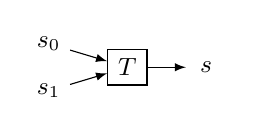
\begin{tikzpicture}[auto,>=latex,minimum width=.5cm]
  \node[] (input0) {$s_0$};
  \node[below of=input0,node distance=.3cm] (dummy) {};
  \node[below of=dummy,node distance=.3cm] (input1) {$s_1$};
  \node[block, right of=dummy] (T) {$T$};
  \node[right of=T] (output) {$s$};
  \draw[->] (input0) -- (T);
  \draw[->] (input1) -- (T);
  \draw[->] (T) -- (output);
\end{tikzpicture}
\end{center}

We generally think of streams as sequences of ``small'' values,
such as insertions or deletions in a database.
However, we also treat the whole database as a \emph{stream of database
snapshots}.  We model a database as a
stream $DB \in \stream{SCH}$, where $SCH$ is the database schema.
Time is not wall-clock time, but counts
the transactions applied to the database.
Since transactions are linearizable, they have a total order.
$DB[t]$ is the snapshot of the
database contents after $t$ transactions have been applied.

Database transactions also form a stream $\Delta DB$, this time a stream of \emph{changes},
or \emph{deltas} that are applied to the database.  The values of
this stream are defined by $(\Delta DB)[t] = DB[t] - DB[t-1]$, where ``$-$'' stands
for the difference between two databases, a notion that we will soon make more precise.
The $\Delta DB$ stream is produced from the $DB$ stream by
the \emph{stream differentiation} operator $\D$;
this operator produces as its output the stream of changes from its input stream;
we have thus $\D(DB) = \Delta DB$.

Conversely, the database snapshot at time $t$ is the cumulative result
of applying all transactions up to $t$: $DB[t] = \sum_{i \leq t}
\Delta DB[i]$.  The operation $\I$, adding up all changes another
basic stream operator, is \emph{stream integration}, the inverse of
differentiation.  The following diagram shows the relationship
between the streams $\Delta DB$ and $DB$:
\begin{center}
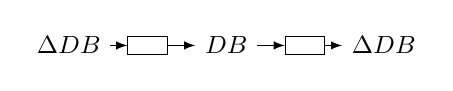
\begin{tikzpicture}[auto,>=latex,minimum width=.5cm]
  \node[] (input) {$\Delta DB$};
  \node[block, right of=input] (I) {$\I$};
  \node[right of=I] (output) {$DB$};
  \node[block, right of=output] (D) {$\D$};
  \node[right of=D] (end) {$\Delta DB$};
  \draw[->] (input) -- (I);
  \draw[->] (I) -- (output);
  \draw[->] (output) -- (D);
  \draw[->] (D) -- (end);
\end{tikzpicture}
\end{center}
Suppose we are given a query $Q : SCH \to SCH$ defining a view $V$.  What is
a view in a streaming model?  It is also a stream!  For each snapshot
of the database stream we have a snapshot of the view: $V[t] = Q(DB[t])$.
In general, given an arbitrary function $f: A \to B$, we define
a streaming ``version'' of $f$, denoted by $\lift{f}$
(read as ``$f$ lifted''), which applies
$f$ to every element of the input stream independently.
We can thus write $V = (\lift{Q})(DB)$.

Armed with these basic definitions, we can precisely define IVM.
What does it mean to maintain a view incrementally?  An
efficient maintenance algorithm needs to compute the \emph{changes} to
the view given the changes to the database. Given a query $Q$, a key
contribution of this paper is the definition of its \emph{incremental
  version} $\inc{Q}$, using stream integration and differentiation:
$\inc{Q} \defn D \circ \lift Q \circ I$. The incremental version of
the query maintains the changes to the view $\Delta V \defn \D(V) =
\D(\lift{Q}(\I(\Delta DB)))$, depicted graphically as:

\begin{center}
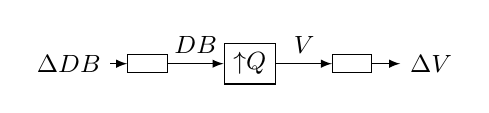
\begin{tikzpicture}[auto,>=latex,minimum width=.5cm]
  \node[] (input) {$\Delta DB$};
  \node[block, right of=input] (I) {$\I$};
  \node[block, right of=I, node distance=1.3cm] (Q) {$\lift{Q}$};
  \node[block, right of=Q, node distance=1.3cm] (D) {$\D$};
  \node[right of=D] (output) {$\Delta V$};
  \draw[->] (input) -- (I);
  \draw[->] (I) -- node (db) {$DB$} (Q);
  \draw[->] (Q) -- node (B) {$V$} (D);
  \draw[->] (D) -- (output);
\end{tikzpicture}
\end{center}

The incremental version of a query is a stateful \emph{streaming
  operator} which computes directly on changes and produces changes.
The incremental version of a query is thus always well-defined.  The
above definition shows one way to compute a query incrementally, but
applying it naively produces an inefficient execution plan, since it
will reconstruct the database at each step.  In
\refsec{sec:incremental} we show how algebraic properties of the
$\inc{\cdot}$ transformation are used to optimize the implementation
of $\inc{Q}$. The first key property is that the incremental
composition of subqueries is the composition of incremental
subqueries: $\inc{(Q_1 \circ Q_2)} = \inc{Q_1} \circ \inc{Q_2}$.  The
second key property is that essentially all primitive database
operations have efficient incremental versions.  More precisely, they
are faster than non-incremental versions by a factor of
$O(|DB|/|\Delta DB|)$.

Armed with this general theory of incremental computation, in
\secref{sec:relational} we show how to model relational queries in
\dbsp.  This immediately gives us a general algorithm to compute the
incremental version of any relational query.  These results were
previously known, but they are cleanly modeled by \dbsp.
\secref{sec:datalog} shows how stratified-monotonic recursive Datalog
programs can be implemented in \dbsp, and \secref{sec:nested} gives
\emph{incremental streaming computations for recursive programs}. For
example, given an implementation of transitive closure in the natural
recursive way, our algorithm produces a program that efficiently
maintains the transitive closure of a graph as the graph is changed by
adding and deleting edges.

In this paper we omits proofs, they can be found in an extensive
companion technical report\anonymize{~\cite{tr}}.  We have formalized
this theory in the Lean proof
assistant~\anonymize{\cite{dbsp-theory}}; our formalization includes
machine-checked proofs of correctness for all the theorems in this
paper.

This paper makes the following contributions:
\begin{enumerate}[nosep, leftmargin=0pt, itemindent=0.5cm, label=\textbf{(\arabic{*})}]
  \item \dbsp, a \textbf{simple} but \textbf{expressive} language for streaming
  computation. \dbsp gives an elegant formal foundation unifying the manipulation of
  streaming and incremental computations.
  \item An algorithm for incrementalizing any streaming computation expressed in
  \dbsp.
  \item An illustration of how \dbsp can model various query classes, such as relational algebra,
  nested relations, aggregations, and stratified-monotonic Datalog.
  \item The first general and machine-checked theory of IVM.
  \item A high-performance open-source implementation of DBSP as a
  general-purpose streaming query engine in Rust.
\end{enumerate}

\section{Stream computations}\label{sec:streams}

The core notion of our theory of IVM is the \textbf{stream}.
In this section we introduce formally streams as
infinite sequences of values, and define computations on streams.
Stream operators (\secref{sec:notation}) are the basic building block of stream
computations.  Operators can be composed with simple rules (\secref{sec:abelian})
into complex computational circuits.
In (\secref{sec:abelianstreams}) we introduce two essential operations on streams:
integration and differentiation.

\subsection{Streams and stream operators}\label{sec:notation}

$\N$ is the set of natural numbers (from 0), $\B$ is the set of
Booleans, $\Z$ is the set of integers, and $\R$ is the set of real
numbers.

\begin{definition}[stream]
Given a set $A$, a \defined{stream} \emph{of values from $A$}, or an
\emph{$A$-stream}, is a function $\N \rightarrow A$.  We denote by
$\stream{A} \defn \{ s \,|\, s : \N \to A \}$ the set of all
$A$-streams.
\end{definition}

When $s\in\stream{A}$ and $t\in\N$ we
write $s[t]$ for the $t$-th element of the stream $s$ instead of the usual $s(t)$.
We think of the index $t\in\N$ as (discrete) time and of $s[t]\in A$
as the value of the the stream $s$ ``at time'' $t$.
\ifstreamexamples
For example, the stream of natural numbers $id \in \stream{\N}$ given by $\id[t] = t$ is the sequence of values
$\sv{0 1 2 3 4}$.
\fi

\begin{definition}[stream operator]
A \defined{stream operator} with $n$ inputs is a function
$T:\stream{A_0}\times\cdots\times\stream{A_{n-1}}\to\stream{B}$.
\end{definition}
In general we use ``operator'' for functions on streams, and
``function'' for computations on ``scalar'' values.

\dbsp is an extension of the simply-typed lambda calculus ---
we will introduce its elements gradually.  However, in many cases we find it more readable to
use circuit diagrams to depict \dbsp programs.
(Circuits do hide the \emph{order} of the inputs of an operator; for non-commutative
operators we have to distinguish the operator inputs.)
In a circuit a rectangle represents an operator application (labeled
with the operator name, e.g., $T$), while an arrow is a stream.

Stream operator \emph{composition} (function composition) is shown as chained circuits.
The composition of a binary operator $T: \stream{A} \times \stream{B} \to \stream{A}$ with the
unary operator $S: \stream{A} \to \stream{B}$ into the computation
$\lambda s. T(T(s,S(s)),S(s)) : \stream{A}\to\stream{A}$
is:

\begin{center}
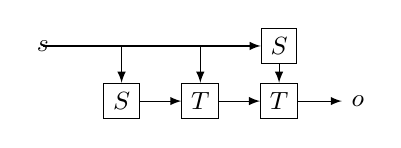
\begin{tikzpicture}[auto,>=latex]
  \node[] (input) {$s$};
  \node[] [right of=input] (dummy) {};
  \node[block, below of=dummy, node distance=.7cm] (S1) {$S$};
  \node[block, right of=S1] (T1) {$T$};
  \node[block, right of=T1] (T2) {$T$};
  \node[block, above of=T2, node distance=.7cm] (S2) {$S$};
  \node[right of=T2] (output) {$o$};
  \draw[->] (input) -| (S1);
  \draw[->] (input) -| (T1);
  \draw[->] (S1) -- (T1);
  \draw[->] (T1) -- (T2);
  \draw[->] (input) |- (S2);  \draw[->] (T2) -- (output);
  \draw[->] (S2) -- (T2);
\end{tikzpicture}
\end{center}


\begin{definition}(lifting)
Given a (scalar) function $f: A \to B$,
we define a stream operator $\lift{f} :\stream{A} \to \stream{B}$
by \emph{lifting} the function $f$ pointwise in time: $(\lift{f})(s) \defn f \circ s$.
Equivalently, $((\lift{f})(s))[t] \defn f(s[t])$.
This extends to functions of multiple arguments.
\end{definition}

\ifstreamexamples
For example, $(\lift{(\lambda x.(2x))})(id) = \sv{0 2 4 6 8}$.
\fi

\begin{proposition}[distributivity]\label{prop:distributivity}
Lifting distributes over function composition:
$\lift{(f \circ g)} = (\lift{f}) \circ (\lift{g})$.
\end{proposition}
\begin{comment}
\begin{proof}
This is easily proved by using associativity of function composition:
$\forall s . (\lift{(f \circ g)})(s) = (f \circ g) \circ s =
f \circ (g \circ s) = f \circ (\lift{g})(s) = (\lift{f})((\lift{g})(s)) =
(\lift{f} \circ \lift{g})(s).$
\end{proof}
\end{comment}

We say that two \dbsp programs are \defined{equivalent} if they compute the same
input-output function on streams.
We use the symbol $\cong$ to indicate that two circuits are
equivalent.  For example, Proposition~\ref{prop:distributivity}
states the following circuit equivalence:

\noindent
\begin{tabular}{m{3.5cm}m{.3cm}m{3.5cm}}
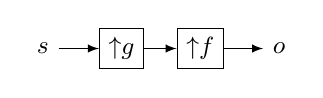
\begin{tikzpicture}[auto,>=latex]
  \node[] (input) {$s$};
  \node[block, right of=input] (g) {$\lift{g}$};
  \node[block, right of=g] (f) {$\lift{f}$};
  \node[right of=f] (output) {$o$};
  \draw[->] (input) -- (g);
  \draw[->] (g) -- (f);
  \draw[->] (f) -- (output);
\end{tikzpicture}
&
$\cong$
&
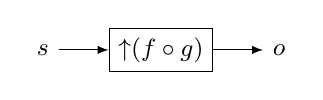
\begin{tikzpicture}[auto,>=latex]
    \node[] (input) {$s$};
    \node[block, right of=input, node distance=1.5cm] (fg) {$\lift{(f \circ g)}$};
    \node[right of=fg, node distance=1.5cm] (output) {$o$};
    \draw[->] (input) -- (fg);
    \draw[->] (fg) -- (output);
\end{tikzpicture}
\end{tabular}

\subsection{Streams over abelian groups}\label{sec:abelian}

For the rest of the technical development we require the set of values
$A$ of a stream $\stream{A}$ to form a commutative group $(A, +, 0_A,
-)$.  The plus defines what it means to add new data, while the minus
allows us to compute differences (deltas); the group structure will
allow us to reorder insertions and deletions.  We show later that this
restriction is not a problem for using \dbsp with relational data.
Now we introduce some useful operators and study their properties.

\subsubsection{Delays and time-invariance}\label{sec:delay}

\begin{definition}[Delay]
The \defined{delay operator}\footnote{The name $\zm$
comes from the DSP literature, and is related to the z-transform~\cite{rabiner-book75}.}
produces an output stream
by delaying its input by one step: $\zm_A: \stream{A} \to \stream{A}$:
%\begin{tabular}{m{5cm}m{3cm}}
$$
\zm_A(s)[t] \defn   \begin{cases}
0_A      & \text{when}~t=0 \\
s[t - 1] & \text{when}~t\geq1
\end{cases}
$$
%&
%\begin{tikzpicture}[auto,node distance=1cm,>=latex]
%    \node[] (input) {$s$};
%    \node[block, right of=input] (z) {$\zm$};
%    \node[right of=z] (output) {$o$};
%    \draw[->] (input) -- (z);
%    \draw[->] (z) -- (output);
%\end{tikzpicture}
%\end{tabular}
\end{definition}

We often omit the type parameter $A$, and write just $\zm$.
\ifstreamexamples
For example, $\zm(\id) = \sv{0 0 1 2 3}$.
\fi

\begin{definition}[Time invariance]
A stream operator $S: \stream{A} \to \stream{B}$ is \defined{time-invariant} (TI) if
$S(\zm_A(s)) = \zm_B(S(s))$ for all $s \in \stream{A}$; in other words, the
if following two circuits are equivalent:

\begin{tabular}{m{3cm}m{.5cm}m{3cm}}
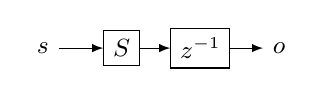
\begin{tikzpicture}[auto,>=latex]
  \node[] (input) {$s$};
  \node[block, right of=input] (S) {$S$};
  \node[block, right of=S] (z) {$\zm$};
  \node[right of=z] (output) {$o$};
  \draw[->] (input) -- (S);
  \draw[->] (S) -- (z);
  \draw[->] (z) -- (output);
\end{tikzpicture}
&
$\cong$
&
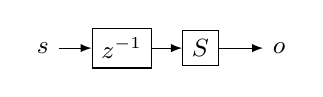
\begin{tikzpicture}[auto,>=latex]
  \node[] (input) {$s$};
  \node[block, right of=input] (z) {$\zm$};
  \node[block, right of=z] (S) {$S$};
  \node[right of=S] (output) {$o$};
  \draw[->] (input) -- (z);
  \draw[->] (z) -- (S);
  \draw[->] (S) -- (output);
\end{tikzpicture}
\end{tabular}

\noindent
This definition extends
naturally to operators with multiple inputs.
\end{definition}

The composition of TI operators of any number of inputs
is TI. The delay operator $\zm$ is TI.
\dbsp only uses TI operators.

%\begin{definition}
%We say that a function between groups $f: A \to B$ has the \emph{zero-preservation
%property} if $f(0_A) = 0_B$.  We write $\zpp{f}$.
%\end{definition}
%
%A lifted operator $\lift{f}$ is TI iff $\zpp{f}$.

\subsubsection{Causal and strict operators}\label{sec:causal}

\begin{definition}[Causality]
A stream operator $S:\stream{A}\to\stream{B}$
is \defined{causal} when for all $s,s'\in\stream{A}$,
and all times $t$ we have:
$
(\forall i \leq t . s[i]=s'[i]) ~~\Rightarrow~~ S(s)[t]=S(s')[t].
$
\end{definition}

\noindent
In other words, the output value at time $t$ can only depend on
input values from times $t' \leq t$.
Operators produced by lifting are causal, and $\zm$ is causal.
All \dbsp operators are causal.  The composition
of causal operators of any number of inputs is causal.

\begin{definition}[Strictness]
A stream operator, $F:\stream{A}\to\stream{B}$
is \defined{strict}
if  $\forall s,s'\in\stream{A}, \forall t \in \N$ we have:
$(\forall i<t . ~s[i]=s'[i]) ~~\Rightarrow \\ F(s)[t]=F(s')[t].$
\end{definition}

In other words, the $t$-th output of $F(s)$ can depend only on ``past'' values
of the input $s$, between $0$ and $t-1$.
In particular, $F(s)[0] = 0_B$ is the same for all $s \in \stream{A}$.
Strict operators are causal. Lifted operators in general are \emph{not} strict.
$\zm$ is strict.  %In \dbsp $\zm$ is the only primitive strict operator.

\begin{proposition}
\label{prop-unique-fix}
For a strict $F: \stream{A} \to \stream{A}$ the equation ~$\alpha=F(\alpha)$~ has a unique
solution $\alpha \in \stream{A}$, denoted by $\fix{\alpha}{F(\alpha)}$.
\end{proposition}

Thus every strict operator from a set to itself has a unique fixed
point.  The simple proof relies on strong induction, showing that the
solution $\alpha[t]$ depends only on the values of $\alpha$ prior to
$t$.

Consider a circuit with a strict feedback edge:
\begin{center}
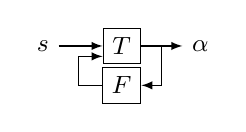
\begin{tikzpicture}[>=latex]
    \node[] (input) {$s$};
    \node[block, right of=input] (f) {$T$};
    \node[right of=f] (output) {$\alpha$};
    \node[block, below of=f, node distance=.5cm] (z) {$F$};
    \draw[->] (input) -- (f);
    \draw[->] (f) -- node (mid) {} (output);
    \draw[->] (mid.center) |-  (z);
    \draw[->] (z.west) -- ++(-.3,0) |- ([yshift=1mm]f.south west);
\end{tikzpicture}
\end{center}

This circuit is a well-defined function on streams:

%\begin{lemma}
%\label{lemma-causal-strict}
%If $F: \stream{B} \to \stream{B}$ is strict and $T: \stream{A} \times \stream{B} \to \stream{B}$ is causal, then for fixed $s$ the operator
%$\lambda\alpha.T(s,F(\alpha)): \stream{A} \to \stream{B}$ is strict.
%\end{lemma}

\begin{lemma}\label{feedback-semantics}
\label{cor-loop}
If $F: \stream{B} \to \stream{B}$ is strict and $T: \stream{A} \times \stream{B} \to \stream{B}$ is causal,
the operator $Q(s)=\fix{\alpha}{T(s,F(\alpha))}$ is well-defined and causal.
If, moreover, $F$ and $T$ are TI then so is $Q$.
\end{lemma}

All \dbsp computations are built using just lifted functions and
delays.  We add two more operators in \secref{sec:nested}.

\subsection{Integration and differentiation}\label{sec:abelianstreams}

Remember that we require the elements of a stream to come from an abelian group $A$.
Streams themselves form an abelian group:

\begin{proposition}
The structure $(\stream{A},+,0,-)$, obtained by lifting the $+$ and unary $-$ operations of $A$,
is an abelian group.  0 is the stream with all values $0_A$.
\end{proposition}

\noindent
Stream addition and negation are causal, TI operators.

\begin{definition}
Given abelian groups $A$ and $B$ we call a stream operator
$S: \stream{A} \rightarrow \stream{B}$ \defined{linear} if it is a group homomorphism, that is,
$S(a+b)=S(a)+S(b)$ (and therefore $S(0)=0$ and $S(-a)=-S(a)$).
\end{definition}

Given a linear function $f: A \to B$, the stream operator $\lift{f}$
is linear and TI (LTI).  $\zm$ is also LTI.

\begin{definition}(bilinear)
A function of two arguments $f: A \times B \to C$ with $A, B, C$ groups, is \emph{bilinear}
if it is linear separately in each argument (i.e., it distributes over addition):
$\forall a, b, c, d . f(a+b, c) = f(a, c) + f(b, c)$, and $f(a, c+d) = f(a, c) + f(c, d).$
\end{definition}

This definition extends to stream operators.
The lifting a bilinear function $f$ is
a bilinear stream operator $\lift{f}$.  An example
is lifted multiplication:
$f: \stream{\N} \times \stream{\N} \to \stream{\N}, f(a, b)[t] = a[t]\cdot b[t]$.

%The composition of (bi)linear operators with linear operators
%is (bi)linear (since homomorphisms compose).

The ``feedback loop'' of a linear operator is linear:

\begin{proposition}
\label{prop-rec-linear}
Let $S$ be a unary, causal, LTI operator. The
operator $Q(s)=\fix{\alpha}{S(s+\zm(\alpha))}$ is well-defined and LTI:

\begin{center}
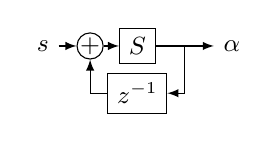
\begin{tikzpicture}[>=latex]
    \node[] (input) {$s$};
    \node[block, shape=circle, right of=input, inner sep=0pt, node distance=.6cm] (plus) {$+$};
    \node[block, right of=plus, node distance=.6cm] (Q) {$S$};
    \node[right of=Q, node distance=1.2cm] (output) {$\alpha$};
    \node[block, below of=Q, node distance=.6cm] (z) {$\zm$};
    \draw[->] (input) -- (plus);
    \draw[->] (plus) -- (Q);
    \draw[->] (Q) -- node (mid) {} (output);
    \draw[->] (mid.center) |-  (z);
    \draw[->] (z) -| (plus);
\end{tikzpicture}
\end{center}
\end{proposition}

\begin{definition}[Differentiation]
The \defined{differentiation operator} $\D_{\stream{A}} : \stream{A} \to \stream{A}$ is defined by:
$\D(s) \defn s - \zm(s)$.

\begin{center}
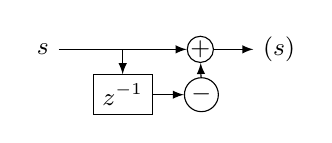
\begin{tikzpicture}[auto,>=latex,node distance=1cm]
    \node[] (input) {$s$};
    \node[block, shape=circle, right of=input, inner sep=0pt,node distance=2cm] (plus) {$+$};
    \node[right of=plus] (output) {$\D(s)$};
    \draw[draw,->] (input) -- node (i) {} (plus);
    \node[block, below of=i, node distance=.7cm] (z) {$\zm$};
    \node[block, shape=circle, right of=z, inner sep=1pt] (minus) {$-$};
    \draw[->] (plus) -- (output);
    \draw[->] (i) -- (z);
    \draw[->] (z) -- (minus);
    \draw[->] (minus) -- (plus);
\end{tikzpicture}
\end{center}
\end{definition}
We generally omit the type, and write just $\D$.
The value of $\D(s)[t] = s[t] - s[t-1]$ if $t > 0$.
\ifstreamexamples
As an example, $\D(\id) = \sv{0 1 1 1 1}$.
\fi

If $s$ is a stream, then $\D(s)$ is the \emph{stream of changes} of $s$.

\begin{proposition}
\label{prop-diff-properties}
$\D$ is causal and LTI.
\end{proposition}

The integration operator ``reconstitutes'' a stream from its changes:

\begin{definition}[Integration]
The \defined{integration operator}  $\I_{\stream{A}} : \stream{A} \to \stream{A}$
is defined by $\I(s) \defn \lambda s . \fix{\alpha}{(s + \zm(\alpha))}$:
\begin{center}
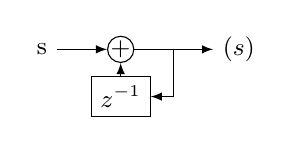
\begin{tikzpicture}[auto,>=latex]
    \node[] (input) {s};
    \node[block, shape=circle, right of=input, inner sep=0pt] (plus) {$+$};
    \node[right of=plus, node distance=1.5cm] (output) {$\I(s)$};
    \node[block, below of=plus, node distance=.6cm] (z) {$z^{-1}$};
    \draw[->] (input) -- (plus);
    \draw[->] (plus) -- node (o) {} (output);
    \draw[->] (o) |- (z);
    \draw[->] (z) -- (plus);
\end{tikzpicture}
\end{center}
\end{definition}

\noindent
We also generally omit the type, and write just $\I$.
This is the construction from Proposition~\ref{prop-rec-linear}
using the identity function for $S$.

\begin{proposition}
$\I(s)$ is the discrete (indefinite) integral applied to the stream $s$:
$\I(s)[t] = \sum_{i \leq t} s[i]$.
\end{proposition}
\ifstreamexamples
As an example, $\I(\id) = \sv{0 1 3 6 10}$.
\fi

\begin{proposition}
\label{prop-integ-properties}
$\I$ is causal and LTI.
\end{proposition}

\begin{theorem}[Inversion]
\label{inverses}
Integration and differentiation are inverses of each other:
$\forall s . \I(\D(s)) = \D(\I(s)) = s$.
\end{theorem}

\noindent
\begin{tabular}{m{2.5cm}m{.3cm}m{1cm}m{.3cm}m{2.5cm}}
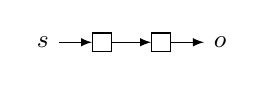
\begin{tikzpicture}[auto,>=latex, node distance=.75cm]
    \node[] (input) {$s$};
    \node[block, right of=input] (I) {$\I$};
    \node[block, right of=I] (D) {$\D$};
    \node[right of=D] (output) {$o$};
    \draw[->] (input) -- (I);
    \draw[->] (I) -- (D);
    \draw[->] (D) -- (output);
\end{tikzpicture}
     &
     $\cong$
     &
     \hspace{-2ex}
\begin{tikzpicture}[auto,>=latex, node distance=.75cm]
    \node[] (input) {$s$};
    \node[right of=input] (output) {$o$};
    \draw[->] (input) -- (output);
\end{tikzpicture}
     &
     $\cong$
     &
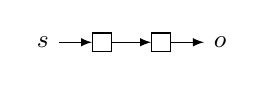
\begin{tikzpicture}[auto,>=latex, node distance=.75cm]
    \node[] (input) {$s$};
    \node[block, right of=input] (D) {$\D$};
    \node[block, right of=D] (I) {$\I$};
    \node[right of=I] (output) {$o$};
    \draw[->] (input) -- (D);
    \draw[->] (D) -- (I);
    \draw[->] (I) -- (output);
\end{tikzpicture}
\end{tabular}

\section{Incremental view maintenance}\label{sec:incremental}

Here we define of IVM and analyze its properties.

\begin{definition}
Given a unary stream operator $Q: \stream{A} \to \stream{B}$ we define the
\defined{incremental version} of $Q$ as:
\begin{equation}\label{def:inc}
\inc{Q} \defn \D \circ Q \circ \I.
\end{equation}
$\inc{Q}$ has the same ``type'' as $Q$: $\inc{Q}: \stream{A} \to \stream{B}$.
For an operator with multiple inputs we define
the incremental version by applying $\I$ to each input independently:
e.g., if $T: \stream{A} \times \stream{B} \rightarrow \stream{C}$ then
$\inc{T}(a, b) \defn \D (T(\I(a), \I(b)))$.
\end{definition}

%The following diagram illustrates the intuition behind this
%definition:
\begin{center}
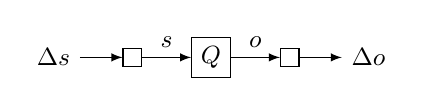
\begin{tikzpicture}[auto,>=latex]
    \node[] (input) {$\Delta s$};
    \node[block, right of=input] (I) {$\I$};
    \node[block, right of=I] (Q) {$Q$};
    \node[block, right of=Q] (D) {$\D$};
    \node[right of=D] (output) {$\Delta o$};
    \draw[->] (input) -- (I);
    \draw[->] (I) -- node (s) {$s$} (Q);
    \draw[->] (Q) -- node (o) {$o$} (D);
    \draw[->] (D) -- (output);
\end{tikzpicture}
\end{center}
If $Q(s) = o$ is a computation, then $\inc{Q}$ performs
the ``same'' computation as $Q$,
but between streams of changes $\Delta s$ and $\Delta o$.

Notice that our definition of incremental computation is meaningful only for \emph{streaming}
computations; this is in contrast to classic definitions, e.g.~\cite{gupta-idb95} which
consider only one change.  Generalizing the definition to operate on streams gives us
additional power, especially when operating with recursive queries.

The following proposition is one of our central results:

\begin{proposition}(Properties of the incremental version):
\label{prop-inc-properties}
\begin{description}[nosep, leftmargin=\parindent]
\item[inversion:] $Q\mapsto\inc{Q}$ is bijective; its inverse is $Q\mapsto \I\circ Q\circ\D$.
\item[invariance:] $\inc{+} = +, \inc{(\zm)} = \zm, \inc{-} = -, \inc{\I}=\I, \inc{\D}=\D$
\item[push/pull:] \label{prop-part-commutation}
    $Q \circ \I = \I \circ \inc{Q}$; $\D\circ Q = \inc{Q}\circ\D$
\item[chain:] $\inc{(Q_1\circ Q_2)} = \inc{Q_1}\circ\inc{Q_2}$ (Generalizes to multiple inputs.)
\item[add:] $\inc{(Q_1 + Q_2)} = \inc{Q_1} + \inc{Q_2}$
\item[cycle:] $\inc{(\lambda s. \fix{\alpha}{T(s,\zm(\alpha)}))} = \lambda s. \fix{\alpha}{\inc{T}(s,\zm(\alpha)})$
\end{description}
\end{proposition}

The \defined{chain rule} states that these two circuits are
equivalent:

\noindent
\begin{tabular}{m{4cm}m{.2cm}m{2.5cm}}
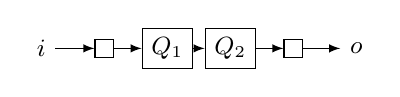
\begin{tikzpicture}[auto,>=latex,node distance=.8cm]
  \node[] (input) {$i$};
  \node[block, right of=input] (I) {$\I$};
  \node[block, right of=I] (Q1) {$Q_1$};
  \node[block, right of=Q1] (Q2) {$Q_2$};
  \node[block, right of=Q2] (D) {$\D$};
  \node[right of=D] (output)  {$o$};
  \draw[->] (input) -- (I);
  \draw[->] (I) -- (Q1);
  \draw[->] (Q1) -- (Q2);
  \draw[->] (Q2) -- (D);
  \draw[->] (D) -- (output);
\end{tikzpicture} &
$\cong$ &
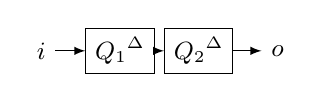
\begin{tikzpicture}[>=latex]
  \node[] (input) {$i$};
  \node[block, right of=input] (Q1) {$\inc{Q_1}$};
  \node[block, right of=Q1] (Q2) {$\inc{Q_2}$};
  \node[right of=Q2] (output)  {$o$};
  \draw[->] (input) -- (Q1);
  \draw[->] (Q1) -- (Q2);
  \draw[->] (Q2) -- (output);
\end{tikzpicture}
\end{tabular}

\noindent In other words, \textbf{to incrementalize a composite query you can incrementalize
each sub-query independently}.  This gives us a simple, syntax-directed, deterministic recipe
for computing the incremental version of an arbitrarily complex query.

The \defined{cycle rule} states that the following circuits are equivalent:

\noindent
\begin{tabular}{m{4.2cm}m{.2cm}m{3cm}}
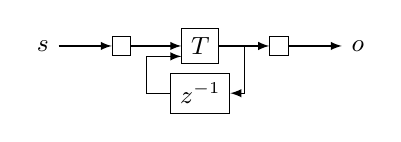
\begin{tikzpicture}[>=latex]
    \node[] (input) {$s$};
    \node[block, right of=input] (I) {$\I$};
    \node[block, right of=I] (f) {$T$};
    \node[block, right of=f] (D) {$\D$};
    \node[right of=D] (output) {$o$};
    \node[block, below of=f, node distance=.6cm] (z) {$\zm$};
    \draw[->] (input) -- (I);
    \draw[->] (I) -- (f);
    \draw[->] (f) -- node (mid) {} (D);
    \draw[->] (mid.center) |-  (z);
    \draw[->] (z.west) -- ++(-.3,0) |- ([yshift=1mm]f.south west);
    \draw[->] (D) -- (output);
\end{tikzpicture} & $\cong$ &
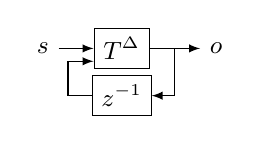
\begin{tikzpicture}[>=latex]
    \node[] (input) {$s$};
    \node[block, right of=input] (f) {$\inc{T}$};
    \node[right of=f, node distance=1.2cm] (output) {$o$};
    \node[block, below of=f, node distance=.6cm] (z) {$\zm$};
    \draw[->] (input) -- (f);
    \draw[->] (f) -- node (mid) {} (output);
    \draw[->] (mid.center) |-  (z);
    \draw[->] (z.west) -- ++(-.3,0) |- ([yshift=1mm]f.south west);
\end{tikzpicture}
\end{tabular}

In other words, the incremental version of a feedback loop around a query
is just the feedback loop with the incremental query for its body.  The significance
of this result will be apparent when we implement recursive queries.

To execute incremental queries efficiently, we want to compute directly
on streams of changes, without integrating them. The invariance property above shows
that stream operators $+$, $-$, and $\zm$ are identical to their incremental versions.
The following theorems generalize this to linear and bi-linear operators:

\begin{theorem}[Linear]\label{linear}
For an LTI operator $Q$ we have $\inc{Q}=Q$.
\end{theorem}

\begin{theorem}[Bilinear]\label{bilinear}
For a bilinear TI operator $\times$ we have
$\inc{(a \times b)} ~=~ a \times b ~+~ \zm(\I(a)) \times b ~+~ a \times \zm(\I(b))
= \I(a) \times b + a \times \zm(\I(b))$.
In pictures: \\
\noindent
\begin{tabular}{m{2.2cm}m{0cm}m{2.3cm}m{0cm}m{2.8cm}}
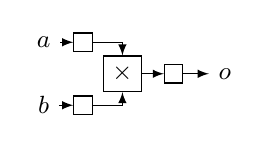
\begin{tikzpicture}[auto,node distance=.65cm,>=latex]
    \node[] (a) {$a$};
    \node[block, right of=a, node distance=.5cm] (ai) {$\I$};
    \node[below of=a, node distance=.4cm] (midway) {};
    \node[below of=midway, node distance=.4cm] (b) {$b$};
    \node[block, right of=b, node distance=.5cm] (bi) {$\I$};
    \node[block, right of=midway, node distance=1cm] (q) {$\times$};
    \node[block, right of=q] (D) {$\D$};
    \node[right of=D] (output) {$o$};
    \draw[->] (a) -- (ai);
    \draw[->] (b) -- (bi);
    \draw[->] (ai) -| (q);
    \draw[->] (bi) -| (q);
    \draw[->] (q) -- (D);
    \draw[->] (D) -- (output);
\end{tikzpicture} &
$\cong$ &
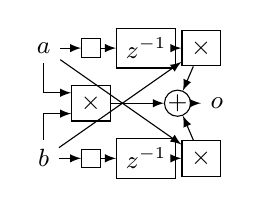
\begin{tikzpicture}[auto,>=latex,node distance=.7cm]
  \node[] (input1) {$a$};
  \node[below of=input1, node distance=1.4cm] (input2) {$b$};
  \node[block, right of=input1, node distance=.6cm] (I1) {$\I$};
  \node[block, below of=I1] (ab) {$\times$};
  \node[block, right of=input2, node distance=.6cm] (I2) {$\I$};
  \draw[->] (input1) -- (I1);
  \draw[->] (input2) -- (I2);
  \draw[->] (input1) |- ([yshift=-1mm]ab.north west);
  \draw[->] (input2) |- ([yshift=1mm]ab.south west);
  \node[block, right of=I1] (ZI1) {$\zm$};
  \node[block, right of=I2] (ZI2) {$\zm$};
  \draw[->] (I1) -- (ZI1);
  \draw[->] (I2) -- (ZI2);
  \node[block, right of=ZI1] (DI1) {$\times$};
  \node[block, right of=ZI2] (DI2) {$\times$};
  \draw[->] (ZI1) -- (DI1);
  \draw[->] (ZI2) -- (DI2);
  \node[block, circle, right of=ab, inner sep=0cm, node distance=1.1cm] (sum) {$+$};
  \draw[->] (ab) -- (sum);
  \draw[->] (DI1) -- (sum);
  \draw[->] (DI2) -- (sum);
  \node[right of=sum, node distance=.5cm] (output) {$o$};
  \draw[->] (sum) -- (output);
  \draw[->] (input1) -- (DI2);
  \draw[->] (input2) -- (DI1);
\end{tikzpicture}
&
$\cong$ &
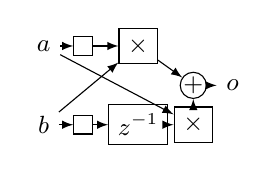
\begin{tikzpicture}[auto,>=latex,node distance=.7cm]
  \node[] (input1) {$a$};
  \node[below of=input1, node distance=1cm] (input2) {$b$};
  \node[block, right of=input1, node distance=.5cm] (I1) {$\I$};
  \node[block, right of=input2, node distance=.5cm] (I2) {$\I$};
  \draw[->] (input1) -- (I1);
  \draw[->] (input2) -- (I2);
  \node[block, right of=I2] (ZI2) {$\zm$};
  \draw[->] (I2) -- (ZI2);
  \node[block, right of=I1] (DI1) {$\times$};
  \node[block, right of=ZI2] (DI2) {$\times$};
  \draw[->] (I1) -- (DI1);
  \draw[->] (ZI2) -- (DI2);
  \node[block, circle, above of=DI2, inner sep=0cm, node distance=.5cm] (sum) {$+$};
  \draw[->] (DI1) -- (sum);
  \draw[->] (DI2) -- (sum);
  \node[right of=sum, node distance=.5cm] (output) {$o$};
  \draw[->] (sum) -- (output);
  \draw[->] (input1) -- (DI2);
  \draw[->] (input2) -- (DI1);
\end{tikzpicture}
\end{tabular}
\end{theorem}

Rewriting Theorem~\ref{bilinear} using $\Delta a$ for the stream of changes to $a$ we
get the familiar formula for incremental equi-joins:
$\Delta(a\times b) =\Delta a \times \Delta b + a\times(\Delta b) +
(\Delta a)\times b$; equi-joins are indeed bilinear.

\section{Relational algebra in \dbsp}\label{sec:relational}

Results in \secref{sec:streams} apply to streams of arbitrary group
values.  In this section we turn our attention to using these results
in the context of relational databases.

However, we face a technical problem: the $\I$ and $\D$ operators were
defined on abelian groups, and relational databases in general are
not abelian groups, since they operate on sets.  Fortunately,
there is a well-known tool in the database literature
which converts set operations into group operations by using \zrs
(also called z-relations~\cite{green-pods07}) instead of sets.

We start by defining the \zrs group, and then we explain how
relational queries are converted into \dbsp circuits over \zrs.

\subsection{\zrs as an abelian group}

Given a set $A$ we define \defined{\zrs}\footnote{Also called $\Z$-relations elsewhere~\cite{green-tcs11}.}
over $A$ as functions with \emph{finite support} from $A$ to $\Z$ (i.e., which are 0 almost everywhere).
These are functions $f: A \rightarrow \Z$ where
$f(x) \not= 0$ for at most a finite number of values $x \in A$.
We also write $\Z[A]$ for the type of \zrs with elements from $A$.
The values in $\Z[A]$ can also be thought as being key-value maps with
keys in $A$ and values in $\Z$, justifying the array indexing notation.

Since $\Z$ is an abelian group, $\Z[A]$ is also an abelian group.  This group
$(\Z[A], +_{\Z[A]}, 0_{\Z[A]}, -_{\Z{A}})$ has addition and subtraction defined pointwise:
$$(f +_{\Z[A]} g)(x) = f(x) + g(x) . \forall x \in A.$$
The $0$ element of $\Z[A]$ is the function $0_{\Z[A]}$ defined by $0_{\Z[A]}(x) = 0 . \forall x \in A$.
(In fact, since $\Z$ is a ring, $\Z[A]$ is also ring, endowed with a multiplication operation,
also defined pointwise.)

A particular \zr $m \in \Z[A]$ can be denoted by enumerating the inputs that map to non-zero values and
their multiplicities:
$m = \{ x_1 \mapsto w_1, \dots, x_n \mapsto w_n \}$.
We call $w_i \in Z$ the \defined{multiplicity} (or weight)
of $x_i \in A$.  Multiplicities can be negative.
We write that $x \in m$ for $x \in A$, iff $m[x] \not= 0$.

For example, let's consider a concrete \zr $R \in \Z[\texttt{string}]$,
defined by $R = \{ \texttt{joe} \mapsto 1, \texttt{anne} \mapsto -1 \}$.
$R$ has two elements in its domain,
\texttt{joe} with a multiplicity of 1 (so $R[\texttt{joe}] = 1$),
and \texttt{anne} with a multiplicity of $-1$.
We say \texttt{joe} $\in R$ and \texttt{anne} $\in R$.

Given a \zr $m \in \Z[A]$ and a value $v \in A$, we overload the array index notation
$m[v]$ to denote the multiplicity of the element $v$ in $m$.
Thus we write $R[\texttt{anne}] = -1$.
When $c \in \Z$, and $v \in A$ we also write $c \cdot v$ for the \defined{singleton} \zr $\{
v \mapsto c \}$.  In other words, $3 \cdot \texttt{frank} = \{ \texttt{frank} \mapsto 3 \}$.
We extend scalar multiplication to operate on \zrs: for $c \in Z, m \in \Z[A]$,
$c \cdot m \defn \sum_{x \in m} (c \cdot m[x]) \cdot x$.  We then have
$2 \cdot R = \{ \texttt{joe} \mapsto 2, \texttt{anne} \mapsto -2 \}$: multiplying
each row weight by 2.

We define the \defined{size} of a \zr as the size of its support set, and we use the
modulus symbol to represent the size: $|m| \defn \sum_{x \in m} 1$.  So $|R| = 2$.

\subsection{Sets, bags, and \zrs}

\zrs generalize sets and bags.
Given a set with elements from $A$, it can be represented as a \zr $\Z[A]$
by associating a weight of 1 with each set element.  The function $\mbox{tozset}: 2^A \to \Z[A]$,
defined as $\mbox{tozset}(s) = \sum_{x \in s} 1 \cdot x$,
converts a set to a \zr by associating a multiplicity of 1 with each set element.
Thus $\mbox{tozset}(\{ \code{joe}, \code{anne} \}) = \{ \code{joe} \mapsto 1, \code{anne} \mapsto 1 \}$.

\begin{definition}
We say that a \zr represents a \defined{set} if the multiplicity of every
element is one.  We define a function to check this property
$\isset : \Z[A] \rightarrow \B$\index{isset}, given by:
$$\isset(m) \defn \left\{
\begin{array}{ll}
  \mbox{true} & \mbox{ if } m[x] = 1, \forall x \in m \\
  \mbox{false} & \mbox{ otherwise}
\end{array}
\right.
$$
\end{definition}
For our example $\isset(R) = \mbox{false}$, since $R[\texttt{anne}] = -1$.
$\isset(\mbox{tozset}(m)) = \mbox{true}$ for any set $m \in 2^A$.

\begin{definition}
We say that a \zr is \defined{positive} (or a \defined{bag}) if the multiplicity of every element is
positive. We define a function to check this property
$\ispositive : \Z[A] \rightarrow \B$\index{ispositive}, given by
$$\ispositive(m) \defn \left\{
\begin{array}{ll}
  \mbox{true} & \mbox{ if } m[x] \geq 0, \forall x \in A \\
  \mbox{false} & \mbox{ otherwise}
\end{array}
\right.$$
\end{definition}
For our example $\ispositive(R) = \mbox{false}$, since $R[\texttt{anne}] = -1$,
but $\isset(m) \Rightarrow \ispositive(m). \forall m \in \Z[A]$.

We also write $m \geq 0$ when $m$ is
positive.  For positive $m, n$ we write $m \geq n$ for $m, n
\in \Z[A]$ iff $m - n \geq 0$.  The relation $\geq$ is a partial order.

\begin{definition}
The function $\distinct: \Z[A] \rightarrow \Z[A]$\index{distinct}
projects a \zr into an underlying set (but \emph{the result is
  still a \zr}).  The definition is $\forall x \in A$
$$\distinct(m)[x] \defn \left\{
\begin{array}{ll}
  1 & \mbox{ if } m[x] > 0 \\
  0 & \mbox{ otherwise}
\end{array}
\right.
$$
\end{definition}
$\distinct(R) = \{ \texttt{joe} \mapsto 1 \}$.

$\distinct$ ``removes'' elements with negative multiplicities.  $\zpp{\distinct}$.

Circuits derived from relational program will only operate with positive \zrs;
non-positive values will be only used to represent \emph{changes} to \zrs
(a change with negative weights will remove elements from a \zr).

\begin{proposition}
$\distinct$ is idempotent: $\distinct = \distinct \circ \distinct$.
\end{proposition}

\begin{proposition}
For any $m \in \Z[A]$ we have: $\isset(\distinct(m))$ and \\
$\ispositive(\distinct(m))$.
\end{proposition}

We call a function $f : \Z[I] \rightarrow \Z[O]$ \defined{positive} if
$\forall x \in \Z[I], x \geq 0_{\Z[I]} \Rightarrow f(x) \geq 0_{\Z[0]}$.
We extend the notation used for \zrs for functions as well: $\ispositive(f)$.

\paragraph{Correctness of the \dbsp implementations}

The function $\mbox{toset}: \Z[A] \to 2^A$, defined as $\mbox{toset}(m) =
\cup_{x \in \distinct(m)} \{ x \}$, converts a \zr into a set.

A relational query $f$ that transforms
a set $V$ into a set $U$ will be implemented by a \dbsp computation $f'$ on
\zrs.  The correctness of the implementation requires that the following
diagram commutes:

\begin{center}
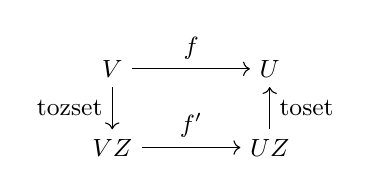
\begin{tikzpicture}
  \node[] (V) {$V$};
  \node[below of=V] (VZ) {$VZ$};
  \node[right of=V, node distance=2cm] (U) {$U$};
  \node[below of=U] (UZ) {$UZ$};
  \draw[->] (V) -- node (f) [above] {$f$} (U);
  \draw[->] (V) --  node (s) [left] {tozset}(VZ);
  \draw[->] (VZ) -- node (f) [above] {$f'$} (UZ);
  \draw[->] (UZ) -- node (d) [right] {toset} (U);
\end{tikzpicture}
\end{center}

\textbf{Remark:} We can generalize the notion of \zrs to functions $m: A \to \mathbf{G}$ for a
ring $\mathbf{G}$ other than $\Z$.  The properties we need from the ring structure are the
following: the ring must be a commutative group (needed for defining $\I$, $\D$, and $\zm$),
the multiplication operation must distribute over addition (needed to define
Cartesian products), and there must be a notion of positive values, needed
to define the $\distinct$ function.  Rings such as $\mathbb{Q}$ or $\mathbb{R}$
would work perfectly.

\subsection{Streams over \zrs}

Since all the results from Section~\ref{sec:streams} are true for streams
over an arbitrary abelian group, they extend to streams where the elements
are \zrs.  In the rest of this text we only consider streams of the form $\stream{\Z[A]}$, for
some element type $A$.

An example of a stream of \zrs is \\ $s = \sv{0 R -1\cdot{R} 2\cdot{R} -2\cdot{R}}$.
We have $s[2] = -R = \{ \texttt{joe} \mapsto -1, \texttt{anne} \mapsto 1 \}$.

\begin{definition}
A stream $s \in \stream{\Z[A]}$ is \defined{positive} if every value of the stream is positive:
$s[t] \geq 0 . \forall t \in \N$.
\end{definition}



\begin{definition}
A stream $s \in \stream{\Z[A]}$ is \defined{monotone} if $s[t] \geq s[t-1], \forall t \in \N$.
\end{definition}

\begin{lemma}
Given a positive stream $s \in \stream{\Z[A]}$ the stream $\I(s)$ is monotone.
\end{lemma}
\begin{proof}
  Let us compute $\I(s)[t + 1] - \I(s)[t] = \sum_{i \leq t+1}s[i] -
  \sum_{i \leq t}s[i] = s[t+1] \geq 0$, by commutativity and positivity of $s$.
\end{proof}

\begin{lemma}
Given a monotone stream $s \in \stream{\Z[A]}$, the
elements of the stream $\D(s)$ are positive.
\end{lemma}
\begin{proof}
  By the definition of monotonicity $s[t+1] \geq s[t]$.  By definition
  of $\D$ we have $\D(s)[t+1] = s[t+1] - s[t] \geq 0$.
\end{proof}

\subsection{Implementing the relational algebra}\label{sec:relational-operators}

The fact that the relational algebra can be implemented by computations
on \zrs has been shown before, e.g.~\cite{green-pods07}.  The translation
of the core relational operators is summarized in Table~\ref{tab:relational} and discussed below.

\begin{table*}
\begin{center}
\footnotesize
\begin{tabular}{|m{1.2cm}m{4.2cm}m{5cm}|} \hline
Operation & SQL example & \dbsp circuit  \\ \hline
Composition &
 \begin{lstlisting}[language=SQL]
SELECT DISTINCT ... FROM
(SELECT ... FROM ...)
\end{lstlisting}
 &
 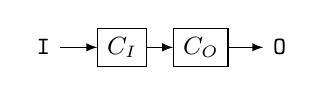
\begin{tikzpicture}[auto,>=latex]
  \node[] (I) {\code{I}};
  \node[block, right of=I] (CI) {$C_I$};
  \draw[->] (I) -- (CI);
  \node[block, right of=CI] (CO) {$C_O$};
  \node[right of=CO] (O) {\code{O}};
  \draw[->] (CI) -- (CO);
  \draw[->] (CO) -- (O);
\end{tikzpicture}
\\ \hline
Union &
\begin{lstlisting}[language=SQL]
(SELECT * FROM I1)
UNION
(SELECT * FROM I2)
\end{lstlisting}
&
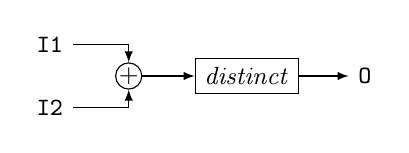
\begin{tikzpicture}[auto,>=latex]
  \node[] (input1) {\code{I1}};
  \node[below of=input1, node distance=.4cm] (midway) {};
  \node[below of=midway, node distance=.4cm] (input2) {\code{I2}};
  \node[block, shape=circle, right of=midway, inner sep=0in] (plus) {$+$};
  \node[block, right of=plus, node distance=1.5cm] (distinct) {$\distinct$};
  \node[right of=distinct, node distance=1.5cm] (output) {\code{O}};
  \draw[->] (input1) -| (plus);
  \draw[->] (input2) -| (plus);
  \draw[->] (plus) -- (distinct);
  \draw[->] (distinct) -- (output);
\end{tikzpicture}
\\ \hline
Projection &
\begin{lstlisting}[language=SQL]
SELECT DISTINCT I.c
FROM I
\end{lstlisting}
&
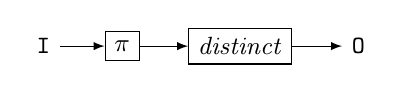
\begin{tikzpicture}[auto,>=latex]
  \node[] (input) {\code{I}};
  \node[block, right of=input] (pi) {$\pi$};
  \node[block, right of=pi, node distance=1.5cm] (distinct) {$\distinct$};
  \node[right of=distinct, node distance=1.5cm] (output) {\code{O}};
  \draw[->] (input) -- (pi);
  \draw[->] (pi) -- (distinct);
  \draw[->] (distinct) -- (output);
\end{tikzpicture}
\\ \hline
Filtering &
\begin{lstlisting}[language=SQL]
SELECT * FROM I
WHERE p(I.c)
\end{lstlisting}
&
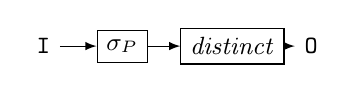
\begin{tikzpicture}[auto,>=latex]
  \node[] (input) {\code{I}};
  \node[block, right of=input] (map) {$\sigma_P$};
  \node[block, right of=map, node distance=1.4cm] (distinct) {$\distinct$};
  \node[right of=distinct] (output) {\code{O}};
  \draw[->] (input) -- (map);
  \draw[->] (map) -- (distinct);
  \draw[->] (distinct) -- (output);
\end{tikzpicture}
\\ \hline
Selection &
\begin{lstlisting}[language=SQL]
SELECT DISTINCT f(I.c, ...)
FROM I
\end{lstlisting}
&
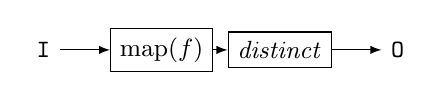
\begin{tikzpicture}[auto,>=latex]
  \node[] (input) {\code{I}};
  \node[block, right of=input, node distance=1.5cm] (map) {$\mbox{map}(f)$};
  \node[block, right of=map, node distance=1.5cm] (distinct) {$\distinct$};
  \node[right of=distinct, node distance=1.5cm] (output) {\code{O}};
  \draw[->] (input) -- (map);
  \draw[->] (map) -- (distinct);
  \draw[->] (distinct) -- (output);
\end{tikzpicture}
\\ \hline
\parbox[b][][t]{1cm}{
Cartesian \\
product} &
\begin{lstlisting}[language=SQL]
SELECT I1.*, I2.*
FROM I1, I2
\end{lstlisting}
&
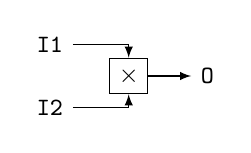
\begin{tikzpicture}[auto,>=latex]
  \node[] (i1) {\code{I1}};
  \node[below of=i1, node distance=.4cm] (midway) {};
  \node[below of=midway, node distance=.4cm] (i2) {\code{I2}};
  \node[block, right of=midway] (prod) {$\times$};
  \node[right of=prod] (output) {\code{O}};
  \draw[->] (i1) -| (prod);
  \draw[->] (i2) -| (prod);
  \draw[->] (prod) -- (output);
\end{tikzpicture}
\\ \hline
Join &
\begin{lstlisting}[language=SQL]
SELECT I1.*, I2.*
FROM I1 JOIN I2
ON I1.c1 = I2.c2
\end{lstlisting}
&
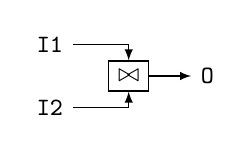
\begin{tikzpicture}[auto,>=latex]
  \node[] (i1) {\code{I1}};
  \node[below of=i1, node distance=.4cm] (midway) {};
  \node[below of=midway, node distance=.4cm] (i2) {\code{I2}};
  \node[block, right of=midway] (prod) {$\bowtie$};
  \node[right of=prod] (output) {\code{O}};
  \draw[->] (i1) -| (prod);
  \draw[->] (i2) -| (prod);
  \draw[->] (prod) -- (output);
\end{tikzpicture}
\\ \hline
Intersection &
\begin{lstlisting}[language=SQL]
(SELECT * FROM I1)
INTERSECT
(SELECT * FROM I2)
\end{lstlisting}
&
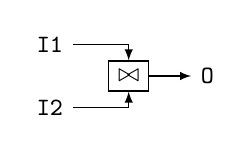
\begin{tikzpicture}[auto,>=latex]
  \node[] (i1) {\code{I1}};
  \node[below of=i1, node distance=.4cm] (midway) {};
  \node[below of=midway, node distance=.4cm] (i2) {\code{I2}};
  \node[block, right of=midway] (prod) {$\bowtie$};
  \node[right of=prod] (output) {\code{O}};
  \draw[->] (i1) -| (prod);
  \draw[->] (i2) -| (prod);
  \draw[->] (prod) -- (output);
\end{tikzpicture}
\\ \hline
Difference &
\begin{lstlisting}[language=SQL]
SELECT * FROM I1
EXCEPT
SELECT * FROM I2
\end{lstlisting}
&
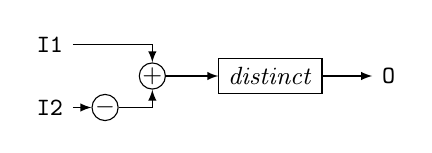
\begin{tikzpicture}[auto,>=latex, node distance=.7cm]
  \node[] (i1) {\code{I1}};
  \node[below of=i1, node distance=.4cm] (midway) {};
  \node[below of=midway, node distance=.4cm] (i2) {\code{I2}};
  \node[block, shape=circle, inner sep=0in, right of=i2] (m) {$-$};
  \node[block, right of=midway, shape=circle, inner sep=0in, node distance=1.3cm] (plus) {$+$};
  \node[block, right of=plus, node distance=1.5cm] (distinct) {$\distinct$};
  \node[right of=distinct, node distance=1.5cm] (output) {\code{O}};
  \draw[->] (i1) -| (plus);
  \draw[->] (i2) -- (m);
  \draw[->] (m) -| (plus);
  \draw[->] (plus) -- (distinct);
  \draw[->] (distinct) -- (output);
\end{tikzpicture}
\\ \hline
\end{tabular}
\caption{Implementation of SQL relational set operators in \dbsp.
Each query assumes that inputs \code{I}, \code{I1}, \code{I2}, are sets and it
produces output sets.\label{tab:relational}}
\end{center}
\end{table*}

The translation is fairly straightforward, but many operators require
the application of a $\distinct$ to produce sets.  The correctness of
this implementation is predicated on the global circuit inputs being
sets as well.

\subsubsection{Query composition}

A composite query is translated by compiling each sub-query separately into a circuit
and composing the respective circuits.

For example, consider the following SQL query:

\begin{lstlisting}[language=SQL]
SELECT ... FROM (SELECT ... FROM ...)
\end{lstlisting}

\noindent given circuits $C_O$ implementing the outer query and $C_I$
implementing the inner query, the translation of the composite query is:

\begin{center}
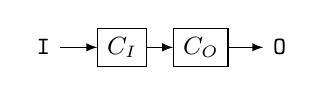
\begin{tikzpicture}[auto,>=latex]
  \node[] (I) {\code{I}};
  \node[block, right of=I] (CI) {$C_I$};
  \draw[->] (I) -- (CI);
  \node[block, right of=CI] (CO) {$C_O$};
  \node[right of=CO] (O) {\code{O}};
  \draw[->] (CI) -- (CO);
  \draw[->] (CO) -- (O);
\end{tikzpicture}
\end{center}

We have $\ispositive(C_I) \land \ispositive(C_0) \Rightarrow \ispositive(C_O \circ C_I)$
and $\zpp{C_I} \land \zpp{C_O} \Rightarrow \zpp{C_O \circ C_I}$.

\subsubsection{Set union}

Consider the following SQL query:

\begin{lstlisting}[language=SQL]
(SELECT * FROM I1) UNION (SELECT * FROM I2)
\end{lstlisting}

The following circuit implements the union program:

\begin{center}
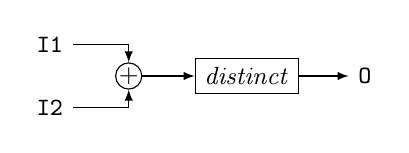
\begin{tikzpicture}[auto,>=latex]
  \node[] (input1) {\code{I1}};
  \node[below of=input1, node distance=.4cm] (midway) {};
  \node[below of=midway, node distance=.4cm] (input2) {\code{I2}};
  \node[block, shape=circle, right of=midway, inner sep=0in] (plus) {$+$};
  \node[block, right of=plus, node distance=1.5cm] (distinct) {$\distinct$};
  \node[right of=distinct, node distance=1.5cm] (output) {\code{O}};
  \draw[->] (input1) -| (plus);
  \draw[->] (input2) -| (plus);
  \draw[->] (plus) -- (distinct);
  \draw[->] (distinct) -- (output);
\end{tikzpicture}
\end{center}

Given \zrs $a, b \in \Z[I]$ s.t. $\isset(a)$ and $\isset(b)$, their \emph{set union}
can be computed as: $\cup: \Z[I] \times \Z[I] \rightarrow \Z[I]$,  $$a
\cup b \defn \distinct(a +_{\Z[I]} b).$$
The $\distinct$ application is necessary to provide the set semantics.

\subsubsection{Projection}
Consider a query such as:

\begin{lstlisting}[language=SQL]
SELECT I.c FROM I
\end{lstlisting}

We can assume without loss of generality that table \code{I} has two columns, and that
a single column is preserved in the projection.
Hence the type of \code{I} is $\Z[A_0 \times A_1]$ while the result has type is $\Z[A_0]$.
In terms of \zrs, the projection of a \zr $i$ on $A_0$ is defined as: $$\pi(i)[y] =
\sum_{x \in i, x|_0 = y} i[x]$$
\noindent where $x|_0$ is first component of the tuple $x$.
In other words, the multiplicity of a tuple in the result is the sum
of the multiplicities of all input tuples that project to it.

The circuit for a projection query is:

\begin{center}
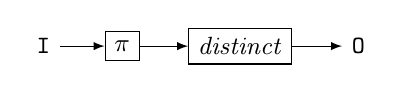
\begin{tikzpicture}[auto,>=latex]
  \node[] (input) {\code{I}};
  \node[block, right of=input] (pi) {$\pi$};
  \node[block, right of=pi, node distance=1.5cm] (distinct) {$\distinct$};
  \node[right of=distinct, node distance=1.5cm] (output) {\code{O}};
  \draw[->] (input) -- (pi);
  \draw[->] (pi) -- (distinct);
  \draw[->] (distinct) -- (output);
\end{tikzpicture}
\end{center}

The $\distinct$ is necessary to convert the result to a set.\\
$\pi$ is linear; $\ispositive(\pi), \zpp{\pi}$.

\subsubsection{Selection}

We generalize the SQL selection operator to allow it to apply an arbitrary function to each row of the
selected set.
Given a function $f : A \rightarrow B$, the mathematical \defined{map} operator ``lifts'' the
function $f$ to operate on \zrs: $\map(f) : \Z[A] \rightarrow \Z[B]$.  A map operator
appears in SQL due to the use of expressions in the SELECT clause, as in the following example:

\begin{lstlisting}[language=SQL]
SELECT f(I.c) FROM I
\end{lstlisting}

The circuit implementation of this query is:

\begin{center}
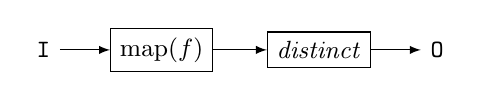
\begin{tikzpicture}[auto,>=latex]
  \node[] (input) {\code{I}};
  \node[block, right of=input, node distance=1.5cm] (map) {$\mbox{map}(f)$};
  \node[block, right of=map, node distance=2cm] (distinct) {$\distinct$};
  \node[right of=distinct, node distance=1.5cm] (output) {\code{O}};
  \draw[->] (input) -- (map);
  \draw[->] (map) -- (distinct);
  \draw[->] (distinct) -- (output);
\end{tikzpicture}
\end{center}

For any function $f$ we have the following properties:
$\map(f)$ is linear, $\ispositive(\map(f)), and \zpp{\map(f)}.$

\subsubsection{Filtering}

Filtering occurs in SQL through a WHERE clause, as in the following example:

\noindent
\begin{lstlisting}[language=SQL]
SELECT * FROM I WHERE p(I.c)
\end{lstlisting}

Let us assume that we are filtering with a predicate
$P: A \rightarrow \B$.  We define the following function $\sigma_P: \Z[A] \rightarrow \Z[A]$ as:
$$\sigma_P(m)[t] = \left\{
\begin{array}{ll}
  m[t] \cdot t & \mbox{ if } P(t) \\
  0 & \mbox{ otherwise } \\
\end{array}
\right.
$$

The circuit for filtering with a predicate $P$ is:

\begin{center}
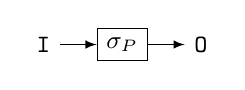
\begin{tikzpicture}[auto,>=latex]
  \node[] (input) {\code{I}};
  \node[block, right of=input] (map) {$\sigma_P$};
  \node[right of=map] (output) {\code{O}};
  \draw[->] (input) -- (map);
  \draw[->] (map) -- (output);
\end{tikzpicture}
\end{center}

For any predicate $P$ we have $\isset(i) \Rightarrow
\isset(\sigma_P(i))$ and $\ispositive(\sigma_P)$.  Thus a $\distinct$
is not needed.  $\sigma_P$ is linear and $\zpp{\sigma_P}$.

\subsubsection{Cartesian products}

Consider this SQL query performing a Cartesian product
between sets \code{I1} and \code{I2}:

\begin{lstlisting}[language=SQL]
SELECT I1.*, I2.* FROM I1, I2
\end{lstlisting}

We first define a product operation on \zrs.
For $a \in \Z[A]$ and $b \in \Z[B]$ we define $a \times b \in \Z[A \times B]$ by
$$(a \times b)((x,y)) \defn a[x] \times b[y] . \forall x \in a, y \in b.$$
The weight of a pair in the result is the product of the weights of the
elements in the sources.  The circuit for the query is:

\begin{center}
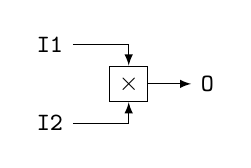
\begin{tikzpicture}[auto,>=latex]
  \node[] (i1) {\code{I1}};
  \node[below of=i1, node distance=.5cm] (midway) {};
  \node[below of=midway, node distance=.5cm] (i2) {\code{I2}};
  \node[block, right of=midway] (prod) {$\times$};
  \node[right of=prod] (output) {\code{O}};
  \draw[->] (i1) -| (prod);
  \draw[->] (i2) -| (prod);
  \draw[->] (prod) -- (output);
\end{tikzpicture}
\end{center}

$\isset(x) \land \isset(y) \Rightarrow \isset(x \times y).$
$\times$ is bilinear, $\ispositive(\times), \zpp{\times}$.

\subsubsection{Joins}

As is well-known, joins can be modeled as Cartesian products
followed by filtering.  Since a join is a composition of a bilinear
and a linear operator, it is also a bilinear operator.
$\ispositive(\bowtie), \zpp{\bowtie}.$

In practice joins are very important computationally, and they are
implemented by a built-in scalar function on \zrs:

$$(a \bowtie b)((x,y)) \defn a[x] \times b[y] \mbox{ if } x|_{c1} = y|_{c2}.$$

\begin{center}
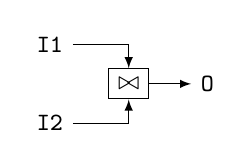
\begin{tikzpicture}[auto,>=latex]
  \node[] (i1) {\code{I1}};
  \node[below of=i1, node distance=.5cm] (midway) {};
  \node[below of=midway, node distance=.5cm] (i2) {\code{I2}};
  \node[block, right of=midway] (prod) {$\bowtie$};
  \node[right of=prod] (output) {\code{O}};
  \draw[->] (i1) -| (prod);
  \draw[->] (i2) -| (prod);
  \draw[->] (prod) -- (output);
\end{tikzpicture}
\end{center}

\subsubsection{Set intersection}

Set intersection is a special case of join, where both relations have the same schema.
It follows that set intersection is bilinear,
and has the zero-preservation property.

\subsubsection{Set difference}  Consider the following query:

\begin{lstlisting}[language=SQL]
SELECT * FROM I1 EXCEPT SELECT * FROM I2
\end{lstlisting}

We define the set difference on \zrs as follows:
$\setminus: \Z[I] \times \Z[I] \rightarrow \Z[I]$, where $$i_1
\setminus i_2 = \distinct(i_1 - i_2).$$  Note
that we have $\forall i_1, i_2, \ispositive(i_1 \setminus
i_2)$ due to the $\distinct$ operator.
The circuit computing the above query is:

\begin{center}
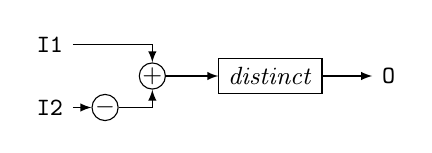
\begin{tikzpicture}[auto,>=latex, node distance=.7cm]
  \node[] (i1) {\code{I1}};
  \node[below of=i1, node distance=.4cm] (midway) {};
  \node[below of=midway, node distance=.4cm] (i2) {\code{I2}};
  \node[block, shape=circle, inner sep=0in, right of=i2] (m) {$-$};
  \node[block, right of=midway, shape=circle, inner sep=0in, node distance=1.3cm] (plus) {$+$};
  \node[block, right of=plus, node distance=1.5cm] (distinct) {$\distinct$};
  \node[right of=distinct, node distance=1.5cm] (output) {\code{O}};
  \draw[->] (i1) -| (plus);
  \draw[->] (i2) -- (m);
  \draw[->] (m) -| (plus);
  \draw[->] (plus) -- (distinct);
  \draw[->] (distinct) -- (output);
\end{tikzpicture}
\end{center}

\section{Recursive queries}\label{sec:recursion}

Recursive queries are very useful in a many applications.
For example, graph algorithms such as graph reachability
or transitive closure are naturally expressed using recursive queries.

We introduce two new simple stream operators that are used for
expressing recursive query evaluation.  These operators allow us
to build circuits implementing looping constructs, which
are used to iterate computations until a fixed-point is reached.

\begin{definition}\label{def:zae}
We say that a stream $s \in \stream{A}$ is \defined{zero almost-everywhere} if it has a finite
number of non-zero values, i.e., there exists a time $t_0 \in \N$
s.t. $\forall t \geq t_0 . s[t] = 0$.
\noindent Denote the set of streams that are zero almost everywhere
by $\streamf{A} \subset \stream{A}$.
\end{definition}

\paragraph{Stream introduction}

The delta function (named from the Dirac delta function) $\delta_0 : A \rightarrow \stream{A}$
produces a stream from a scalar value:
$$\delta_0(v)[t] \defn \left\{
\begin{array}{ll}
  v & \mbox{if } t = 0 \\
  0_A & \mbox{ otherwise}
\end{array}
\right.
$$
\ifstreamexamples
For example, $\delta_0(5)$ is the stream $\sv{5 0 0 0 0}$.
\fi

\begin{comment}
Here is a diagram showing a $\delta_0$ operator; note that the input is a scalar value,
while the output is a stream:

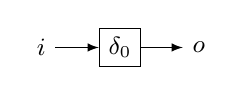
\begin{tikzpicture}[auto,node distance=1cm,>=latex]
    \node[] (input) {$i$};
    \node[block, right of=input] (delta) {$\delta_0$};
    \node[right of=delta] (output) {$o$};
    \draw[->] (input) -- (delta);
    \draw[->] (delta) -- (output);
\end{tikzpicture}
\end{comment}

\paragraph{Stream elimination}

We define the function $\int : \streamf{A} \rightarrow
A$, over streams that are zero almost everywhere, as
$\int(s) \defn \sum_{t \geq 0} s[t]$.
$\int$ is closely related to $\I$; if $\I$ is the
indefinite (discrete) integral, $\int$ is the definite (discrete) integral on the
interval $0 - \infty$.  For example, $\int(\sv{1 2 3 0 0}) = 6$.

For many classes of queries (including
relational and Datalog queries given below) the $\int$
operator can be implemented precisely by integrating until the
first 0 value encountered.

\begin{comment}
Here is a diagram using the $\int$ operator; note that  the result it
produces is a scalar, and not a stream:

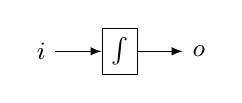
\begin{tikzpicture}[auto,node distance=1cm,>=latex]
    \node[] (input) {$i$};
    \node[block, right of=input] (S) {$\int$};
    \node[right of=S] (output) {$o$};
    \draw[->] (input) -- (S);
    \draw[->] (S) -- (output);
\end{tikzpicture}
\end{comment}

%$\delta_0$ is the left inverse of $\int$, i.e.: $\int \circ \; \delta_0 = \id_A$.
\begin{proposition}
$\delta_0$ and $\int$ are LTI.
\end{proposition}

\paragraph{Nested time domains}

So far we have used a tacit assumption that ``time'' is common for all
streams in a program.  For example, when we add two streams,
we assume that they use the same ``clock'' for the time dimension.
However, the $\delta_0$ operator creates a stream with a ``new'', independent time
dimension.  We require \emph{well-formed circuits}
to ``insulate'' such
nested time domains by ``bracketing'' them between a $\delta_0$
and an $\int$ operator:

\begin{center}
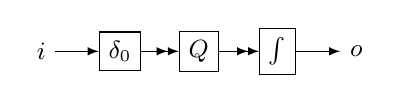
\begin{tikzpicture}[auto,node distance=1cm,>=latex]
    \node[] (input) {$i$};
    \node[block, right of=input] (delta) {$\delta_0$};
    \node[block, right of=delta] (f) {$Q$};
    \draw[->] (input) -- (delta);
    \draw[->>] (delta) -- (f);

    \node[block, right of=f] (S) {$\int$};
    \node[right of=S] (output) {$o$};
    \draw[->>] (f) -- (S);
    \draw[->] (S) -- (output);
\end{tikzpicture}
\end{center}

In this circuit the arrows with double
heads denote stream values, while the simple arrow denote scalar values\footnote{We only use this convention in this diagram;
in general the type of an arrow can be inferred from the type
of its source node.}.  $Q$ is a streaming operator, but the entire circuit is a scalar function.

Algorithm~\ref{algorithm-rec} below, which translates recursive queries to
\dbsp circuits, always produces well-formed circuits.
%\begin{proposition}
%If $Q$ is time-invariant, the circuit above has the zero-preservation
%property: $\zpp{\int \circ\; Q \circ \delta_o}$.
%\end{proposition}

\subsection{Implementing recursive queries}\label{sec:datalog}

We describe the implementation of recursive queries in \dbsp for
stratified Datalog.
In general, a recursive Datalog program defines a set of
mutually recursive relations $O_1,..,O_n$ as an equation
$(O_1,..,O_n)=R(I_1,..,I_m, O_1,..,O_n)$, where $I_1,..,I_m$ are
input relations and $R$ is a relational (non-recursive) query.

We describe the algorithm for
the simpler case of a single-input, single-output query\footnote{The general case
can be found in the companion technical report~\anonymize{\cite{tr}}, and is only
slightly more involved.}.  The input of our algorithm is a Datalog query of the form
$O = R(I, O)$, where $R$ is a relational, non-recursive query,
producing a set as a result, but whose output $O$ is also an input.
The output of the algorithm is a \dbsp circuit which evaluates this
recursive query producing output $O$ when given the input $I$.  Here we build
a non-incremental circuit, which evaluates the Datalog query;
in \refsec{sec:nested} we derive the incremental version
of this circuit.

\begin{algorithm}[recursive queries]\label{algorithm-rec}
\noindent
\begin{enumerate}[nosep, leftmargin=\parindent]
\item Implement the non-recursive relational query $R$ as described in
    \secref{sec:relational} and Table~\ref{tab:relational}; this produces
    an acyclic circuit whose inputs and outputs are a \zrs:
    \begin{center}
    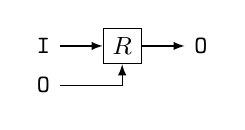
\begin{tikzpicture}[auto,>=latex]
      \node[] (I) {\code{I}};
      \node[below of=I, node distance=.5cm] (O) {\code{O}};
      \node[block, right of=I] (R) {$R$};
      \node[right of=R] (o) {\code{O}};
      \draw[->] (I) -- (R);
      \draw[->] (O) -| (R);
      \draw[->] (R) -- (o);
    \end{tikzpicture}
    \end{center}

\item Lift this circuit to operate on streams:
    \begin{center}
    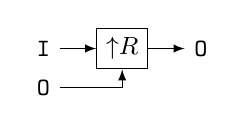
\begin{tikzpicture}[auto,>=latex]
      \node[] (I) {\code{I}};
      \node[below of=I, node distance=.5cm] (O) {\code{O}};
      \node[block, right of=I] (R) {$\lift R$};
      \node[right of=R] (o) {\code{O}};
      \draw[->] (I) -- (R);
      \draw[->] (O) -| (R);
      \draw[->] (R) -- (o);
    \end{tikzpicture}
    \end{center}
  We construct $\lift{R}$ by lifting each operator of the circuit individually
  according to Proposition~\ref{prop:distributivity}.

\item Build a cycle, connecting the output to the corresponding
recursive input via a delay:

 \begin{center}
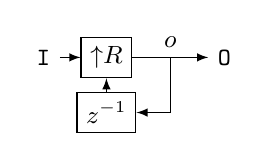
\begin{tikzpicture}[auto,>=latex, node distance=.8cm]
  \node[] (I) {\code{I}};
  \node[block, right of=I] (R) {$\lift R$};
  \node[right of=R, node distance=1.5cm] (O) {\code{O}};
  \node[block, below of=R, node distance=.7cm] (z) {$\zm$};
  \draw[->] (I) -- (R);
  \draw[->] (R) -- node(o) {$o$} (O);
  \draw[->] (o) |- (z);
  \draw[->] (z) -- (R);
 \end{tikzpicture}
 \end{center}
\item ``Bracket'' the circuit in $\I$ and $\D$ nodes, and then in $\delta_0$ and $\int$:

\begin{center}
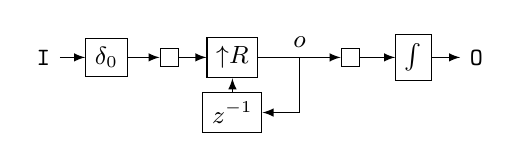
\begin{tikzpicture}[auto,>=latex, node distance=.8cm]
  \node[] (Iinput) {\code{I}};
  \node[block, right of=Iinput] (ID) {$\delta_0$};
  \node[block, right of=ID] (II) {$\I$};
  \node[block, right of=II] (f) {$\lift{R}$};
  \node[block, right of=f, node distance=1.5cm] (D) {$\D$};
  \node[block, right of=D] (S) {$\int$};
  \node[right of=S] (output)  {\code{O}};
  \draw[->] (Iinput) -- (ID);
  \draw[->] (ID) -- (II);
  \draw[->] (II) -- (f);
  \draw[->] (f) -- node (o) {$o$} (D);
  \draw[->] (D) -- (S);
  \draw[->] (S) -- (output);
  \node[block, below of=f, node distance=.7cm] (z) {$\zm$};
  \draw[->] (o) |- (z);
  \draw[->] (z) -- (f);
\end{tikzpicture}
\end{center}
\end{enumerate}
\end{algorithm}

We argue that the cycle inside this circuit computes iteratively the fixed point of $R$.
The $\D$ operator yields the set of new Datalog facts (changes) computed by each iteration of the loop.
When the set of new facts becomes empty, the fixed point has been reached:

\begin{theorem}[Recursion correctness]\label{theorem:recursion}
If $\isset(\code{I})$, the output of the circuit above is
the relation $\code{O}$ as defined by the Datalog semantics of given program
as a function of the input relation \code{I}.
\end{theorem}
\label{proof-recursion}
%\begin{proof}
%Let us compute the contents of the $o$ stream, produced at the output
%of $R$.  We will show that this stream is composed
%of increasing approximations of the value of \code{O}.
%
%Define the following one-argument function: $S(x) = \lambda x . R(\code{I}, x)$.
%Notice that the left input of the $\lift{R}$ block is a constant stream
%with the value \code{I}.  Due to the stratified nature of the language,
%we must have $\ispositive(S)$, so $\forall x . S(x) \geq x$.
%We get the following system of equations:
%$$
%\begin{aligned}
%o[0] =& S(0) \\
%o[t] =& S(o[t-1]) \\
%\end{aligned}
%$$
%So, by induction on $t$ we have $o[t] = S^t(0)$, where by
%$S^t$ we mean $\underbrace{S \circ S \circ \ldots \circ S}_{t}$.
%$S$ is monotone; thus, if there is a time $k$ such that $S^k(0) = S^{k+1}(0)$, we have
%$\forall j \in \N . S^{k+j}(0) = S^k(0)$.  Applying a $\D$ to this stream
%will then produce a stream that is zero almost everywhere, and integrating
%this result will return the last distinct value in the stream $o$.
%
%This is essentially the definition of the semantics of a recursive Datalog relation:
%$\code{O} = \fix{x}{R(\code{I}, x)}$.
%\end{proof}

Note that if the query $R$ computes over unbounded data domains
(e.g., using integers with arithmetic), this construction does
not guarantee convergence.  But if a program does converge,
the above construction will find the least fixed point.

In fact, this circuit implements the standard \defined{na\"{\i}ve evaluation}
algorithm (e.g., see Algorithm~1 in \cite{greco-sldm15}).
Notice that the inner part of the circuit is the incremental
form of another circuit, since it is sandwiched between $\I$ and $\D$ operators.
Using the cycle rule of Proposition~\ref{prop-inc-properties} we can rewrite this circuit as:
%
\begin{equation}
\begin{aligned}
\label{eq:seminaive}
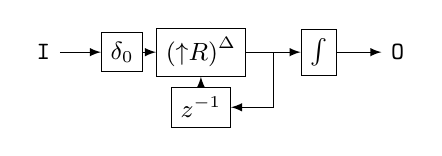
\begin{tikzpicture}[auto,>=latex]
  \node[] (Iinput) {\code{I}};
  \node[block, right of=Iinput] (Idelta) {$\delta_0$};
  \node[block, right of=Idelta] (f) {$\inc{(\lift{R})}$};
  \node[block, right of=f, node distance=1.5cm] (S) {$\int$};
  \node[right of=S] (output)  {\code{O}};
  \node[block, below of=f, node distance=.7cm] (z) {$\zm$};
  \draw[->] (Iinput) -- (Idelta);
  \draw[->] (f) -- node (o) {} (S);
  \draw[->] (S) -- (output);
  \draw[->] (o) |- (z);
  \draw[->] (z) -- (f);
  \draw[->] (Idelta) -- (f);
\end{tikzpicture}
\end{aligned}
\end{equation}

This last circuit effectively implements the \defined{semi-na\"{\i}ve evaluation}
algorithm (Algorithm~2 from~\cite{greco-sldm15}).  We have just proven the correctness
of semi-na\"{\i}ve evaluation as an immediate consequence of the cycle rule.

%In \refsec{sec:recursive-example} we show a concrete example, applying Algorithm~\ref{algorithm-rec}
%to a recursive query computing the transitive closure of a graph.

\section{Incremental recursive programs}\label{sec:nested}

In \secref{sec:streams}--\ref{sec:relational}
we showed how to incrementalize a relational query by
compiling it into a circuit, lifting the circuit to compute on streams, and
applying the $\inc{\cdot}$ operator.  In \secref{sec:recursion} we showed
how to compile a recursive query into a circuit that employs incremental
computation internally (using semi-na\"ive evaluation), to compute the fixed point.
Here we combine these results to construct a circuit that evaluates a \emph{recursive
query incrementally}.  The circuit receives a stream of updates to input
relations, and for every update recomputes the fixed point.  To do this
incrementally, it preserves the stream of changes to recursive relations
produced by the iterative fixed point computation, and adjusts this stream to
account for the modified inputs.  Thus, every element of the input stream yields
a stream of adjustments to the fixed point computation, using
\emph{nested streams}.

Nested streams, or streams of streams, $\stream{\stream{A}} = \N \rightarrow (\N
\rightarrow A)$, are well defined, since streams form an abelian group.
Equivalently, a nested stream is a value in $\N \times \N \to A$, i.e., a matrix
with an infinite number of rows, indexed by two-dimensional time $(t_0, t_1)$.
where each row is a stream.  Please refer to our companion report for
example computations on nested streams~\cite{tr}.

%In the Appendix in
%\secref{sec:nested-examples} we show a few example nested stream
%computations.

Lifting a stream operator $S: \stream{A} \to \stream{B}$ yields an operator over
nested streams $\lift{S}: \stream{\stream{A}} \to \stream{\stream{B}}$, such
that $(\lift{S})(s) = S \circ s$, or, pointwise: $(\lift{S}(s))[t_0][t_1] =
S(s[t_0])[t_1], \forall t_0, t_1 \in \N$.  In particular, a scalar function $f:
A \rightarrow B$ can be lifted twice to produce an operator between streams of
streams: $\lift{\lift{f}}: \stream{\stream{A}} \rightarrow \stream{\stream{B}}$.

To define recursive nested queries, we need a slightly different definition of strictness. If we think of a nested stream $F: \stream{\stream{A}} \to \stream{\stream{B}}$ as a function of timestamps $(i, j)$, then the prior definition of strictness corresponds to strictness in the first dimension $i$, which we extend here to allow $F$ to be strict in its second dimension $j$: for any $s, s' \in \stream{\stream{A}}$ and all times $t \in \N$, $\forall i, j < t.\, s[i][j] = s'[i][j]$ implies $F(s)[i][t] = F(s')[i][t]$.
Proposition~\ref{prop-unique-fix} holds for this extended notion of strictness, i.e., the fixed point operator $\fix{\alpha}{F(\alpha)}$ is well defined for a strict operator $F$.

\begin{proposition}\label{prop-liftz}
The operator $\lift{\zm}: \stream{\stream{A}} \to \stream{\stream{A}}$ is strict (in its second dimension).
\end{proposition}

The operator $\zm$ on nested streams delays ``rows'' of the matrix,
while $\lift{\zm}$ delays ``columns''.
The $\I$ operator on $\stream{\stream{A}}$ operates on rows
of the matrix, treating each row as a single value.
Lifting a stream operator computing on $\stream{A}$,
such as $\I: \stream{A} \to \stream{A}$, also produces an operator on nested streams, but
this time computing on the columns of the matrix
$\lift{\I}: \stream{\stream{A}} \to \stream{\stream{A}}.$

\begin{proposition}[Lifting cycles]
\label{prop-lift-cycle}
For a binary, causal $T$ we have:
$\lift{(\lambda s. \fix{\alpha}{T(s,\zm(\alpha)}))} = \lambda s. \fix{\alpha}{(\lift{T})(s,(\lift{\zm})(\alpha))}$
\noindent i.e., lifting a circuit containing a ``cycle'' can be accomplished by
lifting all operators independently, including the $\zm$ back-edge.
\end{proposition}

This means that lifting a \dbsp stream operator can be expressed within \dbsp
itself.  For example, we have:

\begin{tabular}{m{2cm}m{.5cm}m{4cm}}
\begin{tikzpicture}[>=latex]
  \node[] (input) {$i$};
  \node[block, right of=input] (I) {$\lift{\I}$};
  \node[right of=I] (output)  {$o$};
  \draw[->] (input) -- (I);
  \draw[->] (I) -- (output);
\end{tikzpicture}
& $\cong$ &
\begin{tikzpicture}[>=latex]
  \node[] (input) {$i$};
  \node[block, circle, right of=input, inner sep=0cm] (p) {$+$};
  \node[right of=p, node distance=1.5cm] (output)  {$o$};
  \node[block, below of=p, node distance=.7cm] (z) {$\lift{\zm}$};
  \draw[->] (input) -- (p);
  \draw[->] (p) -- node (mid) {} (output);
  \draw[->] (z) -- (p);
  \draw[->] (mid.center) |- (z);
\end{tikzpicture}
\end{tabular}

This proposition gives the ability to lift
entire circuits, including circuits computing on streams and having feedback edges,
which are well-defined, due to Proposition~\ref{prop-liftz}.
With this machinery we can now apply Algorithm~\ref{algorithm-inc} to arbitrary
circuits, even circuits built for recursively-defined relations.

\noindent Step 1: Start with the ``semi-naive'' circuit~(\ref{eq:seminaive}):
\begin{center}
\begin{tikzpicture}[>=latex]
  \node[] (Iinput) {\code{I}};
  \node[block, right of=Iinput] (Idelta) {$\delta_0$};
  \node[block, right of=Idelta] (f) {$\inc{(\lift{R})}$};
  \node[block, right of=f, node distance=1.5cm] (S) {$\int$};
  \node[right of=S] (output)  {\code{O}};
  \draw[->] (f) -- node (o) {} (S);
  \node[block, below of=o, node distance=.7cm] (z) {$\zm$};
  \draw[->] (Iinput) -- (Idelta);
  \draw[->] (S) -- (output);
  \draw[->] (o.center) -- (z);
  \draw[->] (z) -| (f);
  \draw[->] (Idelta) -- (f);
\end{tikzpicture}
\end{center}
\noindent Step 2: nothing to do (for $\distinct$). \\
\noindent Steps 3 and 4: Lift the circuit (using~\ref{prop-lift-cycle}) and incrementalize:
\begin{center}
\begin{tikzpicture}[>=latex]
  \node[] (Iinput) {$\Delta$\code{I}};
  \node[block, right of=Iinput] (I) {$\I$};
  \node[block, right of=I] (Idelta) {$\lift{\delta_0}$};
  \node[block, right of=Idelta, node distance=1.5cm] (f) {$\lift{\inc{(\lift{R})}}$};
  \node[block, right of=f, node distance=1.5cm] (S) {$\lift{\int}$};
  \node[block, right of=S] (D) {$\D$};
  \node[right of=D] (output)  {$\Delta$\code{O}};
  \draw[->] (f) -- node (o) {} (S);
  \node[block, below of=o, node distance=.7cm] (z) {$\lift{\zm}$};
  \draw[->] (Iinput) -- (I);
  \draw[->] (I) -- (Idelta);
  \draw[->] (S) -- (D);
  \draw[->] (D) -- (output);
  \draw[->] (o.center) -- (z);
  \draw[->] (z) -| (f);
  \draw[->] (Idelta) -- (f);
\end{tikzpicture}
\end{center}

\noindent Step 5: apply the chain rule and linearity of $\lift{\delta_0}$ and $\lift{\int}$:
\begin{equation}
\begin{aligned}
\label{eq:increcursive}
\begin{tikzpicture}[>=latex]
  \node[] (Iinput) {$\Delta$\code{I}};
  \node[block, right of=Iinput] (Idelta) {$\lift{\delta_0}$};
  \node[block, right of=Idelta, node distance=2cm] (f) {$\inc{(\lift{\inc{(\lift{R})}})}$};
  \node[block, right of=f, node distance=2cm] (S) {$\lift{\int}$};
  \node[right of=S] (output)  {$\Delta$\code{O}};
  \draw[->] (f) -- node (o) {} (S);
  \node[block, below of=o, node distance=.7cm] (z) {$\lift{\zm}$};
  \draw[->] (Iinput) -- (Idelta);
  \draw[->] (S) -- (output);
  \draw[->] (o.center) -- (z);
  \draw[->] (z) -| (f);
  \draw[->] (Idelta) -- (f);
\end{tikzpicture}
\end{aligned}
\end{equation}

This is the incremental version of an arbitrary recursive query.  An
example for a transitive closure query is in our report~\cite{tr}.

%\refsec{sec:recursive-incremental-example} shows how Algorithm~\ref{algorithm-inc} is
%applied to the \dbsp circuit produced by the example from~\refsec{sec:recursive-example},
%which implements the recursive query computing the transitive closure of a graph.

\subsection{Cost of incremental recursive queries}

\paragraph{Time complexity}

The time complexity of an incremental recursive query can be estimated as a product of
the number of fixed point iterations and the complexity of each iteration. The
incrementalized circuit (\ref{eq:increcursive}) never performs more
iterations than the non-incremental circuit (\ref{eq:seminaive}):
once the non-incremental circuit reaches the fixed point, its output is constant,
and the derivative of corresponding value in the incrementalized circuit becomes 0.

Moreover, the work performed by each operator in the incremental
circuit is asymptotically less than the non-incremental one.  A
detailed analysis can be found in our companion report~\cite{tr}.

%As a concrete example, consider a join in a recursive circuit.
%A non-incremental implementation is shown in the Appendix in
%example~\ref{recursive-join}.  The incremental implementation
%of the same circuit is in circuit~\ref{join-expansion}, and contains
%4 join operators.  The work performed by the non-incremental join is $O(|DB|^2)$ for
%each iteration.  The size of the inputs of each of the joins in the incremental
%circuit is shown in \ref{sec:work}.  We notice that the four join operators
%perform work $O(|\Delta DB|^2)$, $O(|DB| |\Delta DB|)$, $(O|DB| |\Delta DB|)$,
%and $O(|DB|, 0)$ \leonid{strange notation} respectively (the last operator performs work only in the first iteration),
%so each of them is asymptotically better than the non-incremental version.

\paragraph{Space complexity} Integration ($\I$) and differentiation ($\D$) of a
stream $\Delta s \in \stream{\stream{A}}$ use memory proportional to
$\sum_{t_2}\sum_{t_1}|s[t_1][t_2]|$, i.e., the total size of changes
aggregated over columns of the matrix.  The unoptimized circuit integrates
and differentiates respectively inputs and outputs of the recursive program
fragment.  As we move $\I$ and $\D$ inside the circuit using the chain rule, we
additionally store changes to intermediate streams.  Effectively we cache results of
fixed point iterations from earlier timestamps to update them efficiently as new input changes arrive.
Notice that space usage is proportional to the \emph{number of iterations of the inner loop}
that computes the fixed-point.
Fortunately, many recursive algorithms converge in a relatively small number of steps
(for example, transitive closure requires a number of steps  log(graph diameter).

\section{Additional query languages}\label{sec:extensions}

In this section we describe several query models that go behind stratified Datalog
and show how they can be implemented in \dbsp.

\subsection{Aggregation}\label{sec:aggregation}

Aggregation in SQL applies a function $a$ to a whole set producing a ``scalar''
result with some type $R$: $a: 2^A \to R$.  We convert such aggregation
functions to operate on \zrs, so in \dbsp an aggregation function has
a signature $a: \Z[A] \to R$.  Correctness of the implementation is 
defined as in \refsec{sec:correctness}.

The SQL \texttt{COUNT} aggregation function is implemented on \zrs by $a_\texttt{COUNT} : \Z[A] \to \Z$, which
computes a \emph{sum} of all the element weights: $a_\texttt{COUNT}(s) = \sum_{x \in s} s[x]$.
The SQL \texttt{SUM} aggregation function is implemented on \zrs by $a_\texttt{SUM}: \Z[\R] \to \R$ which
performs a \emph{weighted sum} of all (real) values: $a_\texttt{SUM}(s) = \sum_{x \in s} x \times s[x]$.

With this definition the aggregation functions $a_\texttt{COUNT}$ and $a_\texttt{SUM}$ are in
fact linear transformations between the group $\Z[A]$ and the result group ($\Z$, and $\R$ respectively).

If the output of the \dbsp circuit can be such a ``scalar'' value, then aggregation
with a linear function is simply function application, and thus it is automatically incremental.  However, in general, for composing multiple queries
we require the result of an aggregation to be a singleton \zr (containing a single value),
and not a scalar value.  In this case the aggregation function is implemented in
\dbsp as the composition of the actual aggregation and the 
$\makeset: A \to \Z[A]$ function, 
which converts a scalar value of type $A$ to a singleton \zr, defined as follows:
$\makeset(x) \defn 1 \cdot x$.

In conclusion, the following SQL query: 
\code{SELECT SUM(c) FROM I} 
is implemented as the following circuit:

\begin{tikzpicture}[auto,>=latex]
  \node[] (I) {\code{I}};
  \node[block, right of=I] (pi) {$\pi_\texttt{C}$};
  \node[block, right of=pi] (a) {$a_\texttt{SUM}$};
  \draw[->] (I) -- (pi);
  \draw[->] (pi) -- (a);
  \node[block, right of=a, node distance=1.5cm] (m) {$\makeset$};
  \node[right of=m, node distance=1.4cm] (O) {\code{O}};
  \draw[->] (a) -- (m);
  \draw[->] (m) -- (O); 
\end{tikzpicture}

The lifted incremental version of this circuit is interesting: since $\pi$ 
and $a_\texttt{SUM}$ are linear, they are equivalent to their own incremental 
versions.  Although $\inc{(\lift \makeset)} = \D \circ \lift{\makeset} \circ \I$
cannot be simplified, it is nevertheless efficient, doing only O(1) work per
invocation, since its input and output are singleton values.

An aggregation function such as \texttt{AVG} can be written as the composition of 
a more complex linear function that computes a pair of values using 
\texttt{SUM} and \texttt{COUNT}, followed by a $\mbox{makeset}$ and a selection operation
that divides the two columns.

\begin{lstlisting}[language=SQL]
SELECT AVG(c) FROM I 
\end{lstlisting}

\begin{tikzpicture}[>=latex]
  \node[] (I) {\code{I}};
  \node[block, right of=I] (pi) {$\pi_\texttt{C}$};
  \node[block, right of=pi, node distance=1.8cm] (sc) {$(a_\texttt{SUM}, a_\texttt{COUNT})$};
  \draw[->] (I) -- (pi);
  \draw[->] (pi) -- (sc);
  \node[block, right of=sc, node distance=2cm] (m) {$\makeset$};
  \node[block, right of=m, node distance=1.4cm] (div) {$\sigma_/$};
  \node[right of=div] (O) {\code{O}};
  \draw[->] (sc) -- (m);
  \draw[->] (m) -- (div);
  \draw[->] (div) -- (O);
\end{tikzpicture}

Finally, some aggregate functions, such as \code{MIN}, are 
\emph{not} incremental in general, since for handling deletions
they may need to know the full set, and not just its changes.  The lifted
incremental version of such aggregate functions is implemented essentially
by ``brute force'', using the formula $\inc{(\lift a_\texttt{MIN})}
= \D \circ \lift{a_\texttt{MIN}} \circ \I$.  Such functions perform work
proportional to $R(s)$ at each invocation.

Note that the SQL \code{ORDER BY} directive can be modeled as
a non-linear aggregate function that emits a list.  However, such an implementation it is not efficiently incrementalizable in \dbsp. 
We leave the efficient handling of ORDER BY to future work.

Even when aggregation results do not form a group, they usually form
a structure with a zero element.  We expect that a well-defined
aggregation function maps empty \zrs to zeros in the target domain.


\subsection{Nested relations}

\subsubsection{Indexed partitions}

Let $A[K]$ be the set of functions with finite support from $K$ to $A$.
Consider a group $A$, an arbitrary set of \defined{key values} $K$, and a 
\emph{partitioning function} $k: A \to A[K]$ with the property that 
$\forall a \in A . a = \sum k(a)$.  We call elements of $A[K]$ \emph{indexed}
values of $A$ --- indexed by a key value.

Notice that $A[K]$ also has a group structure, and $k$ itself 
is a linear function (homomorphism).  As an example,
if $A = \Z[B_0 \times B_1]$, we can use for $k$ the first projection
$k: A \to \Z[A][B_0]$, where $k(a)[b] = \sum_{t \in a, t|0 = b} a[t] \cdot t$.
In other words, $k$ projects the elements in $\Z[B_0 \times B_1]$ on 
their first component.  This enables \emph{incremental computations
on nested relations}.  This is how operators such as group-by are
implemented: the result of group-by is an indexed \zr, where each 
element is indexed by the key of the group it belongs to.  Since
indexing is linear, its incremental version is very efficient.
Notice that the structure $\Z[A][K]$ represents a form of \emph{nested relation}.

\subsection{Grouping; indexed relations}\label{sec:grouping}

Pick an arbitrary set $K$ of ``key values.''
Consider the mathematical structure of finite maps from $K$ 
to \zrs over some other domain $A$: $K \to \Z[A] = \Z[A][K]$.
We call values $i$ of this structure \defined{indexed \zrs}: for
each key $k \in K$, $i[k]$ is a \zr.  Because 
the codomain $\Z[A]$ is an abelian group, this structure is itself 
an abelian group.

We use this structure to model the SQL \texttt{GROUP BY} operator in \dbsp.  
Consider a \defined{partitioning function}
$p: A \to K$ that assigns a key to any value in $A$.  We define the grouping function
$G_p: \Z[A] \to (K \to \Z[A])$ as $G_p(a)[k] \defn \sum_{x \in a.p(x)=k}a[x] \cdot x$.
When applied to a \zr $a$ this function returns a indexed \zr, where each element 
is called a \defined{grouping}\footnote{We use
``group'' for the algebraic structure and ``grouping'' for the result of \code{GROUP BY}.}: for each key $k$ a 
grouping is a \zr containing all elements of $a$ that map to $k$ 
(as in SQL, groupings are multisets, represented by \zrs).
Consider our example \zr $R$ from \refsec{sec:relational},
and a key function $p(s)$ that returns the first letter of the string 
$s$. Then we have that $G_p(R) = \{ \code{j} \mapsto \{ \code{joe} 
\mapsto 1 \}, \code{a} \mapsto \{ \code{anne} \mapsto -1 \} \}$,
i.e., grouping with this key function produces an indexed \zr with two groupings, each 
of which contains a \zr with one element.

The grouping function $G_p$ is linear for any $p$.
It follows that the group-by implementation in DBSP is automatically
incremental: given some changes
to the input relation we can apply the partitioning function
to each change separately to compute how each grouping changes.

\subsection{\texttt{GROUP BY-AGGREGATE}}

Grouping in SQL is almost always followed by aggregation.  
Let us consider an aggregation function $a: (K \times \Z[A]) \to B$ that produces values
in some group $B$, and an indexed relation of type $\Z[A][K]$, as defined above in~\refsec{sec:grouping}.
The nested relation aggregation operator $Agg_a: \Z[A][K] \to B$ applies $a$ 
to the contents of each grouping independently and adds the results:
$Agg_a(g) \defn \sum_{k \in K} a(k, g[k])$.  To apply this
to our example, let us compute the equivalent of GROUP-BY count; we use
the following aggregation function $count: K \times \Z[A]$, $count(k, s) = 
\makeset((k, a_\texttt{COUNT}(s)))$, using the \zr counting function $a_\texttt{COUNT}$ 
from~\refsec{sec:aggregation}; the notation $(a,b)$ is a pair of values $a$ and $b$.
Then we have $Agg_{count} (G_p(R)) = \{ (\code{j}, 1) \mapsto 1, 
(\code{a}, -1) \mapsto 1 \}$.

Notice that, unlike SQL, \dbsp can express naturally computations
on indexed \zrs, they are just an instance of a group structure. 
One can even implement queries that operate on each grouping 
in an indexed \zr.  However, our definition of incremental 
computation is only concerned with incrementality in the 
\emph{outermost} structures.  We leave it to future work to
explore an appropriate definition of incremental computation that
operates on the \emph{inner} relations.

A very useful operation on nested relations is \defined{flatmap}, which is
essentially the inverse of partitioning, converting an indexed
\zr into a \zr: $\mbox{flatmap}: \Z[A][K] \to \Z[A \times K]$.
$\mbox{flatmap}$ is in fact a particular instance of aggregation,
using the aggregation function $a: K \times \Z[A] \to \Z[A \times K]$
defined by $a(k, s) = \sum_{x \in s[k]} s[k][x] \cdot (k, x).$
For our previous example, $\mbox{flatmap}(G_p(R)) = \{ (\code{j}, \code{joe}) \mapsto 1, 
(\code{a}, \code{anne}) \mapsto -1 \}$.

If we use an aggregation function $a: K \times Z[A]$ that is linear in its
second argument, then the aggregation operator $Agg_a$ is linear, and
thus fully incremental.  As a consequence, $\mbox{flatmap}$ is linear.  
However, many practical aggregation functions for nested relations are in fact 
not linear; an example is the $count$ function above, which is not linear
since it uses the $\makeset$ non-linear function.  Nevertheless, while 
the incremental evaluation of such functions is not fully incremental, 
it is at least partly incremental: when applying a change to groupings, the aggregation 
function only needs to be re-evaluated \emph{for groupings that have changed}.


\subsection{Streaming joins}

Consider a binary query $T(s, t) = \I(t)~~\lift{\bowtie}~~s$.  This is the
\emph{relation-to-stream join} operator supported by streaming databases like ksqlDB~\cite{jafarpour-edbt19}.
Stream $t$ carries changes to a relation, while $s$ carries arbitrary data, e.g., logs
or telemetry data points. $T$ ``discards'' values from $s$ after matching them against the accumulated contents of the relation.

\begin{center}
\noindent
\begin{tikzpicture}[>=latex]
  \node[] (t) {$t$};
  \node[below of=t] (s) {$s$};
  \node[right of=t, block] (I) {$\I$};
  \node[below of=t, node distance=.5cm] (mid) {};
  \node[block, right of=mid, node distance=2cm] (j) {$\bowtie$};
  \node[right of=j] (o) {$o$};
  \draw[->] (s) -| (j);
  \draw[->] (t) -- (I);
  \draw[->] (I) -| (j);
  \draw[->] (j) -- (o);
\end{tikzpicture}
\end{center}

\subsection{Explicit delay}

So far the $\zm$ operator was confined to its implicit use in integration or
differentiation.  However, it can be exposed as a primitive operation that
can be applied to streams or collections.  This enables programs that can
perform time-based window computations over streams, and convolution-like
operators.  


\subsection{Multisets/bags}

Since \zrs generalize multisets and bags, it is easy to implement query
operators that compute on such structures.  For example, while SQL \code{UNION}
is \zr addition followed by $\distinct$, \code{UNION ALL} is just \zr addition.


\subsection{Window aggregates}

Streaming databases often organize the contents of streams into windows, 
which store a subset of data points with a predefined range of timestamps.
The circuit below (a convolution filter in DSP) computes a \emph{fixed-size sliding-window aggregate}
over the last four timestamps defined by the $T_i$ functions.

\begin{center}
\begin{tikzpicture}[>=latex]
    \node[] (input) {$s$};
    \node[block, right of=input, node distance=1.5cm] (f0) {$T_0$};
    \node[below of=input, node distance=1cm] (fake) {};
    \node[block, right of=fake, node distance=1cm] (z0) {$\zm$};
    \node[right of=input, node distance=.35cm] (tap) {};
    \node[block, right of=f0, node distance=1.5cm] (f1) {$T_1$};
    \node[block, right of=z0, node distance=1.2cm] (z1) {$\zm$};
    \node[block, right of=f1, node distance=1.5cm] (f2) {$T_2$};
    \node[block, right of=z1, node distance=1.5cm] (z2) {$\zm$};
    \draw[->] (input) -- (f0);
    \draw[->] (tap.center) |- (z0);
    \draw[->] (z0) -| (f0);
    \draw[->] (f0) -- (f1);
    \draw[->] (z0) -- (z1);
    \draw[->] (z1) -| (f1);
    \draw[->] (f1) -- (f2);
    \draw[->] (z1) -- (z2);
    \draw[->] (z2) -| (f2);
    \node[right of=f2] (output) {$o$};
    \draw[->] (f2) -- (output);
\end{tikzpicture}
\end{center}

In practice, windowing is usually based on physical timestamps attached to
stream values rather than logical time.  For instance, the CQL~\cite{arasu-tr02} query
``\texttt{SELECT * FROM events [RANGE 1 hour]}'' returns all events received
within the last hour.  The corresponding circuit (on the left) takes input stream $s \in \stream{\Z[A]}$ and an additional
input $\theta \in \stream{\mathbb{R}}$ that carries the value of the current
time.

\begin{tabular}{m{3cm}m{0.5cm}m{3cm}}
\begin{tikzpicture}[>=latex]
    \node[] (input) {$s$};
    \node[above of=input, node distance=.5cm] (t) {$\theta$};
    \node[block, right of=input] (i) {$I$};
    \node[block, right of=i] (w) {$W$};
    \node[right of=w] (output) {$o$};
    \draw[->] (input) -- (i);
    \draw[->] (i) -- (w);
    \draw[->] (w) -- (output);
    \draw[->] (t) -| (w);
\end{tikzpicture}
&
$\cong$
&
\begin{tikzpicture}[>=latex]
    \node[] (input) {$s$};
    \node[above of=input, node distance=.5cm] (t) {$\theta$};
    \node[block, shape=circle, right of=input, inner sep=0pt] (plus) {$+$};
    \node[block, right of=plus] (w) {$W$};
    \node[right of=w] (output) {$o$};
    \node[block, below of=plus, node distance=.8cm] (z) {$\zm$};
    \draw[->] (input) -- (plus);
    \draw[->] (plus) -- (w);
    \draw[->] (t) -| (w);
    \draw[->] (w) -- node (mid) {} (output);
    \draw[->] (mid.center) |-  (z);
    \draw[->] (z) -- (plus);
\end{tikzpicture} \\
\end{tabular}

\noindent{}where the \emph{window operator} $W$ prunes input \zrs, only keeping values
with timestamps less than an hour behind $\theta[t]$.  Assuming $ts: A \to \mathbb{R}$ returns
the physical timestamp of a value, $W$ is defined as $W(v, \theta)[t] \defn \{x \in v[t] . 
ts(x) \geq \theta[t] - 1hr\}$.  Assuming $\theta$ increases monotonically, $W$
can be moved inside integration, resulting in the circuit on the right, which uses
bounded memory to compute a window of an unbounded stream.
This circuit is a building block of a large family of window queries, including
window joins and aggregation.  We conjecture that \dbsp can express 
any CQL query.

\begin{center}
\begin{tikzpicture}[>=latex]
  \node[] (input) {$i$};
  \node[right of=input] (invisible) {};
  \node[block, right of=invisible] (A) {$A$};
  \node[block, above of=invisible, node distance=.7cm] (S) {$S$};
  \node[block, circle, right of=S, inner sep=0cm] (m) {$-$};
  \node[block, circle, right of=A, inner sep=0cm] (p) {$+$};
  \node[right of=p, node distance=1.5cm] (output)  {$w$};
  \node[block, below of=p, node distance=.7cm] (z) {$\zm$};
  \draw[->] (input) -- (A);
  \draw[->] (input) |- (S);
  \draw[->] (A) -- (p);
  \draw[->] (p) -- node (mid) {} (output);
  \draw[->] (mid.center) |- (z);
  \draw[->] (S) -- (m);
  \draw[->] (m) -| (p);
  \draw[->] (z) -| (S);
  \draw[->] (z) -| (A);
\end{tikzpicture}
\end{center}

\subsection{Relational while queries}
(See also non-monotonic semantics for Datalog$^\neg$ and Datalog$^{\neg\neg}$\cite{Abiteboul-book95}.)
To illustrate the power of \dbsp we implement the following
``while'' program, where $Q$ is an arbitrary relational algebra query:
{\small
\begin{lstlisting}[language=Pascal]
x := i;
while (x changes)
    x := Q(x);
\end{lstlisting}}
The \dbsp implementation of this program is:

%$$\lambda i. \int[\D[\fix{\xi}{Q(\delta_0(i)+\zm(\xi))}]]$$
\begin{center}
\begin{tikzpicture}[>=latex]
  \node[] (input) {$i$};
  \node[block, right of=input] (delta) {$\delta_0$};
  \node[block, circle, right of=delta, inner sep=0cm] (p) {$+$};
  \node[block, right of=p] (Q) {$\lift Q$};
  \node[block, right of=Q] (D) {$\D$};
  \node[block, right of=D] (S) {$\int$};
  \node[right of=S] (output)  {$x$};
  \node[block, below of=p, node distance=.7cm] (z) {$\zm$};
  \draw[->] (input) -- (delta);
  \draw[->] (delta) -- (p);
  \draw[->] (p) -- (Q);
  \draw[->] (Q) -- node (mid) {} (D);
  \draw[->] (D) -- (S);
  \draw[->] (mid.center) |- (z);
  \draw[->] (S) -- (output);
  \draw[->] (z) -- (p);
\end{tikzpicture}
\end{center}

This circuit can be converted to a streaming circuit that computes a stream of values $i$ 
by lifting it; it can be incrementalized using Algorithm~\ref{algorithm-inc} to compute on changes of $i$:

\begin{center}
\begin{tikzpicture}[>=latex]
  \node[] (input) {$\Delta i$};
  \node[block, right of=input] (delta) {$\lift{\delta_0}$};
  \node[block, circle, right of=delta, inner sep=0cm] (p) {$+$};
  \node[block, right of=p] (Q) {$\inc{(\lift{\lift{Q}})}$};
  \node[block, right of=Q, node distance=1.5cm] (D) {$\lift{\D}$};
  \node[block, right of=D, node distance=1.1cm] (S) {$\lift{\int}$};
  \node[right of=S, node distance=1.2cm] (output)  {$\Delta x$};
  \node[block, below of=p, node distance=.9cm] (z) {$\lift{\zm}$};
  \draw[->] (input) -- (delta);
  \draw[->] (delta) -- (p);
  \draw[->] (p) -- (Q);
  \draw[->] (Q) -- node (mid) {} (D);
  \draw[->] (D) -- (S);
  \draw[->] (mid.center) |- (z);
  \draw[->] (S) -- (output);
  \draw[->] (z) -- (p);
\end{tikzpicture}
\end{center}


\section{Implementation}\label{sec:implementation}

We are prototyping an implementation of \dbsp as part of an
open-source project with an MIT license: 
\url{https://github.com/vmware/database-stream-processor}.
The implementation is written in Rust.
The implementation consists of a library and a runtime.
The library provides APIs for basic algebraic data types:
such as groups, finite maps, \zr, indexed \zr.  
A separate circuit construction API allows users to 
create \dbsp circuits by placing operator nodes (corresponding to boxes in our diagrams)
and connecting them with streams, which correspond to the
arrows in our diagrams.  The library provides pre-built generic operators
for integration, differentiation, delay, nested integration and differentiation.
The \zr library provides functions for computing the basic \zr operations
corresponding to plus, negation, grouping, joining, aggregation.

For iterative computations we provide the $\delta_0$ operator and
an operator that approximates $\int$ by terminating iteration of
a loop at a user-specified condition (usually the condition is the 
requirement for a zero to appear in a specified stream).
The low level library allows users to construct incremental
circuits manually.  Our plan is to add a higher-level library
(a compiler) which will automatically incrementalize a circuit.

\section{Additional Implementation Details}\label{sec:implementation-additional}

\subsection{Checkpoint/restore}

DDlog programs are stateful streaming systems.  Fault-tolerance and 
migration for such programs requires state migration.  We claim that it is 
sufficient to checkpoint and restore the "contents" of all $\zm$ operator
in order to migrate the state of a Ddlog computation.

\subsection{Maintaining a database}

DDlog is not a database, it is just a streaming view maintenance system.
In particular, DDlog will not maintain more state than absolutely necessary
to compute the changes to the views.  There is no way to find out whether 
a specific value exists at a specific time moment within a DDlog relation.
However, a simple extension to DDlog runtime can be made to provide a \emph{view query}
API: essentially all relations that may be queried have to be maintained 
internally in an integrated form as well.  The system can then provide
an API to enumerate or query a view about element membership between 
input updates.

\subsection{Materialized views}

An incremental view maintenance system is not a database -- it only computes changes
to views when given changes to tables.  However, it can be integrated with a 
database, by providing capabilities for \emph{querying} both tables and views.
An input table is just the integral of all the changes to the table.  This makes
possible building a system that is both stateful (like a database) and streaming
(like an incremental view maintenance system).

\subsection{Maintaining input invariants}

For relational query systems there is however an important caveat: 
the proofs about the correctness
of the $C_Q$ implementing the same semantics as $Q$ all require some 
preconditions on the circuit inputs.  In particular, the semantics of $Q$
is only defined for sets.  In order for $C_Q$ to faithfully emulate
the behavior of $Q$ we must enforce the invariant that the input
relations are in fact sets.  

However, the differential streaming version of the circuits accepts
an arbitrary stream of changes to the input relations.  Not all
such streams define input relations that are sets!  For example,
consider an input stream where the first element removes a
tuple from an input relation.  The resulting \zr does not represent
a set, and thus the proof of correctness does not hold.
This problem has been well understood in the context of the
relational algebra: it is the same as the notion of positivity from~\cite{green-tcs11}.

We propose three different solutions to this problem, in increasing degrees of complexity.

\paragraph{Assume that the environment is well-behaved}

The simplest solution is to do nothing and assume that at any point in time 
the integral of the input stream of changes $i$ is a set: $\forall t \in \N . \isset(\I(i)[t])$.
This may be a reasonable assumption if the changes come from a controlled
medium, e.g., a traditional database, where they represent legal database changes.

\paragraph{Normalize input relations to sets}

In order to enforce that the input relations are always sets it is sufficient
to apply a $\distinct$ operator after integration.  

\begin{tikzpicture}[auto,node distance=1cm,>=latex]
    \node[] (input) {$i$};
    \node[block, right of=input] (I) {$\I$};
    \node[block, right of=I, node distance=1.5cm] (distinct) {$\distinct$};
    \node[block, right of=distinct, node distance=1.5cm] (q) {$\lift{C_Q}$};
    \node[block, right of=q] (D) {$\D$};
    \node[right of=D] (output) {$o$};
    \draw[->] (input) -- (I);
    \draw[->] (I) -- (distinct);
    \draw[->] (distinct) -- (q);
    \draw[->] (q) -- (D);
    \draw[->] (D) -- (output);
\end{tikzpicture}

The semantics of the resulting circuit is identical to the semantics of $\inc{\lift{C_Q}}$
for well-behaved input streams.  For non-well behaved input streams one can give
a reasonable definition: a change is applied to the input relations, and then non-relations
are normalized into relations.  Removing a non-existent element is a no-op, and adding twice
an element is the same as adding it once.

\paragraph{Use a ``change manager''}

In this solution we interpose a separate software component between the environment
and the circuit.  Let us call this a ``change manager'' (CM).  The CM
is responsible for accepting commands from the environment that perform updates on the input
relations, validating them, and building incrementally an input change, by computing the
effect of the commands.  The CM needs to maintain enough internal state to validate all commands; this 
will most likely entail maintaining the full contents of the input tables.  Note that
the input tables can be computed as the $\I$ of all input deltas ever applied.  Once all 
commands producing a change have been accepted, the environment can apply the produced input change
atomically, and obtain from the circuit the corresponding output changes.

\begin{tikzpicture}[auto,node distance=1cm,>=latex]
    \node[minimum width=.5cm, minimum height=1cm] (env) {Env};
    \node[block, right of=env, minimum width=.5cm, minimum height=1cm, node distance=1.5cm] (tm) {CM};
    \node[block, right of=tm, node distance=1.5cm] (C) {$\inc{\lift{C_Q}}$};
    \node[right of=C] (output) {$o$};
    \draw[->] (env.30) -- (tm.150);
    \draw[<-] (env.330) -- (tm.210);
    \draw[->] (tm) -- node (i) {$i$} (C);
    \draw[->] (C) -- (output);
\end{tikzpicture}
\section{Related work}\label{sec:related}

\subsection{Incremental View Maintenance}

Incremental view maintenance~\cite{gupta-sigmod93, griffin-sigmod95, chaudhuri-icde95,
gupta-idb95, chirkova-book12} is a much studied problem in databases.
A survey of results for Datalog queries is present in~\cite{motik-ai19}.
The standard approach is as follows: given a query $Q$, discover a ``delta query'',
a``differential'' version $\Delta Q$ that satisfies the equation:
$Q(d+\Delta d)=Q(d)+\Delta Q(d,\Delta d)$, and which can be used to compute
the change for a new input reusing the previous output.
DBToaster introduced recursive recursive IVM~\cite{ahmad-vldb09, koch-pods10}, where
the incrementalization process is repeated for the delta query.

Many custom algorithms were published for various classes of queries: e.g.~\cite{koch-pods16}
handles positive nested relational calculus.  DYN~\cite{idris-sigmod17}
and IDYN~\cite{idris-vldb18, idris-sigmod19} focus on acyclic conjunctive queries.  Instead
of keeping the output view materialized they build data structures that allow efficiently
querying the output views.  PAI maps~\cite{abeysinghe-sigmod22} are specially
designed for queries with correlated aggregations.
AJU~\cite{wang-sigmod20} focuses on foreign-key joins.  It is a matter
of future work to evaluate whether custom \dbsp operators
can match the efficiency of systems specialized for narrow classes
of queries.

\dbsp is a bottom-up system, which always produces eagerly
the\emph{changes} to the output views.
Instead of maintaining the output view entirely, \dbsp proposes
generating deltas as the output of the computation (similar to the kSQL~\cite{jafarpour-edbt19}
\texttt{EMIT CHANGES} queries).  The idea that both
inputs and outputs to an IVM system are streams of changes
seems trivial, but this is key to the symmetry of our solution:
both in our definition of IVM~(\ref{def:inc}), and the fundamental
reason that the chain rule exists --- the chain rule is the one that makes our
structural induction IVM algorithm possible.

IVM algorithms for Datalog-like languages frequently use counting based
approaches~\cite{Dewan-iis92,motik-aaai15} that maintain the number of derivations of each
output fact: DRed~\cite{gupta-sigmod93} and its variants~\cite{Ceri-VLDB91,Wolfson-sigmod91,%
Staudt-vldb96,Kotowski-rr11,Lu-sigmod95,Apt-sigmod87}, the backward-forward algorithm
and variants~\cite{motik-aaai15,Harrison-wdd92,motik-ai19}.
\dbsp is more general than these approaches,
and our incrementalization algorithm handles arbitrary recursive queries and
generates more efficient plans for recursive queries
in the presence of arbitrary updates (especially deletions, where competing approaches
may over-delete).  Interestingly, the \zrs multiplicities in \dbsp are related
to the counting-number-of-derivations approaches, but our use of the $\distinct$
operator shows that precise counting is not necessary.

Picallo et al.~\cite{picallo-scop19} provide a general solution to IVM for
rich languages.  \dbsp requires a group structure on the values operated on;
this assumption has two major practical benefits: it simplifies the mathematics considerably
(e.g., Picallo uses monoid actions to model changes), and it provides a general, simple
algorithm (\ref{algorithm-inc}) for incrementalizing arbitrary programs.  The downside of
\dbsp is that one has to find a suitable group structure (e.g., \zrs for sets) to ``embed''
the computation.  Picallo's notion of ``derivative'' is not unique: they need creativity to choose
the right derivative definition, we need creativity to find the right group structure.

Finding a suitable group structure has proven easy for relations (both~\cite{koch-pods10}
and~\cite{green-tcs11} use \zrs to uniformly model data and insertions/deletions), but it is
not obvious how to do it for other data types, such as sorted collections, or tree-shaped
collections (e.g., XML or JSON documents)~\cite{foster-planx08}.  An intriguing question
is ``what other interesting group structures could this be applied to besides \zrs?''
Papers such as~\cite{nikolic-icmd18} explore other possibilities, such as matrix algebra,
linear ML models, or conjunctive queries.

\dbsp does not do anything special for triangle queries~\cite{kara-tds20}.  Are there
better algorithms for this case?

In \secref{sec:extensions} we have briefly mentioned that \dbsp can easily
model window and stream database queries~\cite{arasu-tr02,aurora}; it is an
interesting question whether there are CQL queries that cannot be expressed in \dbsp
(we conjecture that there aren't any).

\begin{comment}
The main problem that change structures address is that the types used in programs are not
closed under subtraction (e.g., the delta between two sets is not a set).
Although a relational \dbsp circuit computes
only on positive \zr values, its incremental version may compute on negative
values, but the equivalence of the two programs guarantees correctness even though the
type system of \zrs does not.  \val{Safe to delete this para}
\end{comment}


\dbsp is also related to Differential Dataflow
(DD)~\cite{mcsherry-cidr13, murray-sosp13} and its theoretical
foundations~\cite{abadi-fossacs15} (and
recently~\cite{mchserry-vldb20,chothia-vldb16}).  DD's computational
model is more powerful than \dbsp, since it allows past values in a
stream to be "updated".  In fact, DD is the only other framework which
we are aware of which can incrementalize recursive queries as
efficiently as \dbsp does.  In contrast, our model assumes that the
inputs of a computation arrive in the time order while allowing for
nested time domains via the modular lifting transformer ($\lift{}$).
\dbsp can express both incremental and non-incremental computations;
in essence \dbsp is ``deconstructing'' DD into simple component
building blocks.  Most importantly, \dbsp comes with
Algorithm~\ref{algorithm-inc}, a syntax-directed translation that can
convert any expressible query into an incremental version --- in DD
users have to assemble incremental queries manually using incremental
operators.  (materialize.com offers a product that automates
incrementalization, but only for SQL queries.  Differential
Datalog~\cite{ryzhyk-datalog19} does it for a Datalog dialect.)
Unlike DD, \dbsp is a modular theory, which easily accommodates the
addition of new operators.  In particular, we have given full
mechanical proofs of \dbsp's correctness.

\subsection{Stream computation models}

\dbsp using non-nested streams is a simplified instance of a Kahn
network~\cite{kahn-ifip74}.  Johnson~\cite{johnson-phd83} studies a
very similar computational model without nested streams and its
expressiveness. The implementation of such streaming models of
computation and their relationship to dataflow machines has been
studied by Lee~\cite{lee-ieee95}.  Lee~\cite{lee-ifip93} also
introduced streams of streams and the $\lift{\zm}$ operator.

\cite{gammie-acs13} surveys the connection between synchronous digital
circuits and functional programs.  Our circuits are nothing but higher
order functions computing on streams (functions themselves).  The
paper's main focus are circuits processing numeric data, whereas,
taking advantage of our circuits' ability to compute on arbitrary
groups, we use circuits to implement incremental view maintenance for
relational databases.

Mamouras~\cite{mamouras-esop20} gives a formal theory of stream computation.

\subsection{Connection to synchronous circuits}

There is a vast literature on \defined{synchronous circuits}, which
are well-defined models for hardware circuits
e.g.~\cite{gammie-acs13}.  These circuits also compute over infinite
streams of values, usually of Booleans $\stream{\B}$.  In a
\defined{combinational circuit} the output values depend only on the
current input values.  These are pure lifted streaming computations.
A \defined{sequential circuit} can have outputs that depend on past
input values.  These are always causal circuits.  Sequential
synchronous circuits use latches or flip-flops to store state; the
latches are controlled by a global clock signal.  These correspond to
the $\zm$ operator.  In a well-formed sequential circuit all
back-edges must go through some latch --- this corresponds to our
circuit construction rule that requires a delay element on each
back-edge.

Languages such as Verilog or VHDL can be used to specify such
circuits.  (However, both Verilog and VHDL are strictly more powerful,
and can express richer classes of circuits than just synchronous
sequential circuits.)

There is a rich literature on synchronous circuits, and some of these
results are directly applicable to the circuits we discuss.  Here are
a few examples.

Retiming~\cite{leiserson-algorithmica91} is an optimization that
``moves'' around delay elements while preserving the circuit
semantics.  Retiming is used traditionally to reduce the clock cycle
by minimizing the signal propagation delay between any pair of
latches.  In our case it could be used for minimizing the amount of
internal circuit state.

In a synchronous circuit the \emph{state} is entirely stored in the
latches.  Saving and restoring the contents of the latches enables
such circuits to take a snapshot of their state and resume
computation.\footnote{In Boolean synchronous circuits this is achieved
  by connecting all latches into a \emph{scan chain} which can be read
  and written sequentially after stopping the circuit clock.}

Fault tolerance of synchronous circuits is provided by replicating the
state elements, to prevent accidental state changes caused by e.g.,
cosmic rays.  We can borrow this idea for building redundant
distributed computations.

Pipelining digital circuits is an effective technique for increasing
throughput through parallelization, by inserting additional latches
and allowing different pipeline stages to compute concurrently on
distinct stream values, at the expense of increased latency between
the inputs and the corresponding outputs.

Digital circuit latches depend on a special ``reset'' signal to
initialize their state to a pre-established value; this corresponds to
the special 0 value in our value domain.

Our nested streams are related to the notion of delta-cycles in the
definition of VHDL~\cite{baker-date96}.

\section{Conclusions}\label{sec:conclusions}%\label{sec:ddlog}

We have introduced \dbsp, a model of computation based on 
infinite streams over abelian groups.  In this model streams are used for 3 purposes:
(1) to model consecutive snapshots of a database, (2) to model consecutive changes (deltas,
or transactions) applied to a database and changes of a maintained view, (3) to model consecutive values of loop-carried variables in recursive computations.

We have defined an abstract notion of incremental computation over streams, 
and defined the incrementalization operator
$\inc{\cdot}$, which transforms an \emph{arbitrary} stream computation $Q$ 
into its incremental version $\inc{Q}$.
The incrementalization operator has some very nice algebraic properties, which
gave us a general algorithm for incrementalizing many classes of complex queries,
including arbitrary recursive queries.

We believe that \dbsp can form a solid foundation for a theory and practice of 
streaming incremental computation.

\bibliographystyle{ACM-Reference-Format}
\bibliography{main}

%\appendix
%\section{Supporting material}\label{sec:extra}

\subsection{Relational Query Example}\label{sec:relational-example}

We apply the IVM algorithm~\ref{algorithm-inc} to a concrete
relational SQL query:
\begin{lstlisting}[language=SQL,basicstyle=\small]
CREATE VIEW v AS
SELECT DISTINCT a.x, b.y FROM (
     SELECT t1.x, t1.id FROM t1 WHERE t1.a > 2
) a JOIN (
     SELECT t2.id, t2.y FROM t2 WHERE t2.s > 5
) b ON a.id = b.id
\end{lstlisting}

Step 1: Create a \dbsp circuit to represent this query using the
translation rules from Table~\ref{tab:relational}; notice that
this circuit is essentially a dataflow implementation of the query.
(Notice that the query asks for \code{SELECT DISTINCT}, so there is a
$\distinct$ operator after $\sigma$):

\noindent
\begin{tikzpicture}[node distance=1.2cm,>=latex]
    \node[] (t1) {\code{t1}};
    \node[block, right of=t1, node distance=.9cm] (s1) {$\sigma_{a > 2}$};
    \node[block, right of=s1] (d1) {$\distinct$};
    \node[block, right of=d1] (p1) {$\pi_{x, id}$};
    \node[block, right of=p1] (d11) {$\distinct$};
    \node[below of=t1, node distance=1cm] (t2) {\code{t2}};
    \node[block, right of=t2, node distance=.9cm] (s2) {$\sigma_{s > 5}$};
    \node[block, right of=s2] (d2) {$\distinct$};
    \node[block, right of=d2] (p2) {$\pi_{y, id}$};
    \node[block, right of=p2] (d21) {$\distinct$};
    \node[below of=d11, node distance=.5cm] (mid) {};
    \node[block, right of=mid, node distance=.8cm] (j) {$\bowtie_{id = id}$};
    \node[block, right of=j] (p) {$\pi_{x, y}$};
    \node[block, right of=p] (d) {$\distinct$};
    \node[right of=d, node distance=.9cm] (V) {\code{V}};
    \draw[->] (t1) -- (s1);
    \draw[->] (s1) -- (d1);
    \draw[->] (d1) -- (p1);
    \draw[->] (p1) -- (d11);
    \draw[->] (t2) -- (s2);
    \draw[->] (s2) -- (d2);
    \draw[->] (d2) -- (p2);
    \draw[->] (p2) -- (d21);
    \draw[->] (d11) -| (j);
    \draw[->] (d21) -| (j);
    \draw[->] (j) -- (p);
    \draw[->] (p) -- (d);
    \draw[->] (d) -- (V);
\end{tikzpicture}

Step 2: apply the rules to eliminate $\distinct$ operators.
First from Proposition~\ref{prop-distinct-once}:

\noindent
\begin{tikzpicture}[node distance=1.2cm,>=latex]
    \node[] (t1) {\code{t1}};
    \node[block, right of=t1, node distance=.9cm] (s1) {$\sigma_{a > 2}$};
    \node[block, right of=s1] (p1) {$\pi_{x, id}$};
    \node[block, right of=p1] (d11) {$\distinct$};
    \node[below of=t1, node distance=1cm] (t2) {\code{t2}};
    \node[block, right of=t2, node distance=.9cm] (s2) {$\sigma_{s > 5}$};
    \node[block, right of=s2] (p2) {$\pi_{y, id}$};
    \node[block, right of=p2] (d21) {$\distinct$};
    \node[below of=d11, node distance=.5cm] (mid) {};
    \node[block, right of=mid, node distance=.8cm] (j) {$\bowtie_{id = id}$};
    \node[block, right of=j] (p) {$\pi_{x, y}$};
    \node[block, right of=p] (d) {$\distinct$};
    \node[right of=d, node distance=.9cm] (V) {\code{V}};
    \draw[->] (t1) -- (s1);
    \draw[->] (s1) -- (p1);
    \draw[->] (p1) -- (d11);
    \draw[->] (t2) -- (s2);
    \draw[->] (s2) -- (p2);
    \draw[->] (p2) -- (d21);
    \draw[->] (d11) -| (j);
    \draw[->] (d21) -| (j);
    \draw[->] (j) -- (p);
    \draw[->] (p) -- (d);
    \draw[->] (d) -- (V);
\end{tikzpicture}

\noindent The rule from Proposition~\ref{prop-distinct-delay} gives
(from now on we omit the subscripts to save space):

\noindent
\begin{tikzpicture}[node distance=1.2cm,>=latex]
    \node[] (t1) {\code{t1}};
    \node[block, right of=t1, node distance=.9cm] (s1) {$\sigma$};
    \node[block, right of=s1] (p1) {$\pi$};
    \node[below of=t1, node distance=1cm] (t2) {\code{t2}};
    \node[block, right of=t2, node distance=.9cm] (s2) {$\sigma$};
    \node[block, right of=s2] (p2) {$\pi$};
    \node[below of=p1, node distance=.5cm] (mid) {};
    \node[block, right of=mid, node distance=.8cm] (j) {$\bowtie$};
    \node[block, right of=j] (d0) {$\distinct$};
    \node[block, right of=d0] (p) {$\pi$};
    \node[block, right of=p] (d) {$\distinct$};
    \node[right of=d, node distance=.9cm] (V) {\code{V}};
    \draw[->] (t1) -- (s1);
    \draw[->] (s1) -- (p1);
    \draw[->] (t2) -- (s2);
    \draw[->] (s2) -- (p2);
    \draw[->] (p1) -| (j);
    \draw[->] (p2) -| (j);
    \draw[->] (j) -- (d0);
    \draw[->] (d0) -- (p);
    \draw[->] (p) -- (d);
    \draw[->] (d) -- (V);
\end{tikzpicture}

\noindent And again~\ref{prop-distinct-once}:

\noindent
\begin{tikzpicture}[node distance=1cm,>=latex]
    \node[] (t1) {\code{t1}};
    \node[block, right of=t1, node distance=.9cm] (s1) {$\sigma$};
    \node[block, right of=s1] (p1) {$\pi$};
    \node[below of=t1, node distance=1cm] (t2) {\code{t2}};
    \node[block, right of=t2, node distance=.9cm] (s2) {$\sigma$};
    \node[block, right of=s2] (p2) {$\pi$};
    \node[below of=p1, node distance=.5cm] (mid) {};
    \node[block, right of=mid, node distance=.8cm] (j) {$\bowtie$};
    \node[block, right of=j] (p) {$\pi$};
    \node[block, right of=p] (d) {$\distinct$};
    \node[right of=d, node distance=1cm] (V) {\code{V}};
    \draw[->] (t1) -- (s1);
    \draw[->] (s1) -- (p1);
    \draw[->] (t2) -- (s2);
    \draw[->] (s2) -- (p2);
    \draw[->] (p1) -| (j);
    \draw[->] (p2) -| (j);
    \draw[->] (j) -- (p);
    \draw[->] (p) -- (d);
    \draw[->] (d) -- (V);
\end{tikzpicture}

At this point no more $\distinct$ elimination rules can be applied.

Step 3: we lift the circuit using distributivity of composition over
lifting (Proposition~\ref{prop:distributivity}); we obtain a circuit
that computes over streams, i.e., for each new input pair of relations
\code{t1} and \code{t2} it will produce an output view \code{V}:

\noindent
\begin{tikzpicture}[node distance=1cm,>=latex]
    \node[] (t1) {\code{t1}};
    \node[block, right of=t1, node distance=.9cm] (s1) {$\lift{\sigma}$};
    \node[block, right of=s1] (p1) {$\lift{\pi}$};
    \node[below of=t1, node distance=1cm] (t2) {\code{t2}};
    \node[block, right of=t2, node distance=.9cm] (s2) {$\lift{\sigma}$};
    \node[block, right of=s2] (p2) {$\lift{\pi}$};
    \node[below of=p1, node distance=.5cm] (mid) {};
    \node[block, right of=mid, node distance=.8cm] (j) {$\lift{\bowtie}$};
    \node[block, right of=j] (p) {$\lift{\pi}$};
    \node[block, right of=p, node distance=1.2cm] (d) {$\lift{\distinct}$};
    \node[right of=d] (V) {\code{V}};
    \draw[->] (t1) -- (s1);
    \draw[->] (s1) -- (p1);
    \draw[->] (t2) -- (s2);
    \draw[->] (s2) -- (p2);
    \draw[->] (p1) -| (j);
    \draw[->] (p2) -| (j);
    \draw[->] (j) -- (p);
    \draw[->] (p) -- (d);
    \draw[->] (d) -- (V);
\end{tikzpicture}

Step 4: incrementalize circuit, obtaining a circuit that computes over changes;
this circuit receives changes to relations \code{t1} and \code{t2} and for each
such change it produces the corresponding change in the output view \code{V}:

\noindent
\begin{tikzpicture}[node distance=1cm,>=latex]
    \node[] (t1) {$\Delta$\code{t1}};
    \node[block, right of=t1, node distance=.8cm] (I1) {$\I$};
    \node[block, right of=I1, node distance=.9cm] (s1) {$\lift{\sigma}$};
    \node[block, right of=s1] (p1) {$\lift{\pi}$};
    \node[below of=t1, node distance=1cm] (t2) {$\Delta$\code{t2}};
    \node[block, right of=t2, node distance=.8cm] (I2) {$\I$};
    \node[block, right of=I2, node distance=.9cm] (s2) {$\lift{\sigma}$};
    \node[block, right of=s2] (p2) {$\lift{\pi}$};
    \node[below of=p1, node distance=.5cm] (mid) {};
    \node[block, right of=mid, node distance=.7cm] (j) {$\lift{\bowtie}$};
    \node[block, right of=j] (p) {$\lift{\pi}$};
    \node[block, right of=p, node distance=1.2cm] (d) {$\lift{\distinct}$};
    \node[block, right of=d, node distance=1.1cm] (D) {$\D$};
    \node[right of=D, node distance=.8cm] (V) {$\Delta$\code{V}};
    \draw[->] (t1) -- (I1);
    \draw[->] (I1) -- (s1);
    \draw[->] (s1) -- (p1);
    \draw[->] (t2) -- (I2);
    \draw[->] (I2) -- (s2);
    \draw[->] (s2) -- (p2);
    \draw[->] (p1) -| (j);
    \draw[->] (p2) -| (j);
    \draw[->] (j) -- (p);
    \draw[->] (p) -- (d);
    \draw[->] (d) -- (D);
    \draw[->] (D) -- (V);
\end{tikzpicture}

Step 5: apply the chain rule to rewrite the circuit as a composition of incremental operators;

\noindent
\begin{tikzpicture}[node distance=1.6cm,>=latex]
    \node[] (t1) {$\Delta$\code{t1}};
    \node[block, right of=t1, node distance=1.2cm] (s1) {$\inc{(\lift{\sigma})}$};
    \node[block, right of=s1] (p1) {$\inc{(\lift{\pi})}$};
    \node[below of=t1, node distance=1.2cm] (t2) {$\Delta$\code{t2}};
    \node[block, right of=t2, node distance=1.2cm] (s2) {$\inc{(\lift{\sigma})}$};
    \node[block, right of=s2] (p2) {$\inc{(\lift{\pi})}$};
    \node[below of=p1, node distance=.6cm] (mid) {};
    \node[block, right of=mid, node distance=.8cm] (j) {$\inc{(\lift{\bowtie})}$};
    \node[block, right of=j] (p) {$\inc{(\lift{\pi})}$};
    \node[block, right of=p] (d) {$\inc{(\lift{\distinct})}$};
    \node[right of=d, node distance=1.2cm] (V) {$\Delta$\code{V}};.8
    \draw[->] (t1) -- (s1);
    \draw[->] (s1) -- (p1);
    \draw[->] (t2) -- (s2);
    \draw[->] (s2) -- (p2);
    \draw[->] (p1) -| (j);
    \draw[->] (p2) -| (j);
    \draw[->] (j) -- (p);
    \draw[->] (p) -- (d);
    \draw[->] (d) -- (V);
\end{tikzpicture}

Use the linearity of $\sigma$ and $\pi$ to simplify this circuit (notice that
all linear operators no longer have a $\inc{\cdot}$):

\noindent
\begin{tikzpicture}[node distance=1cm,>=latex]
    \node[] (t1) {$\Delta$\code{t1}};
    \node[block, right of=t1, node distance=1cm] (s1) {$\lift{\sigma}$};
    \node[block, right of=s1] (p1) {$\lift{\pi}$};
    \node[below of=t1, node distance=1.2cm] (t2) {$\Delta$\code{t2}};
    \node[block, right of=t2, node distance=1cm] (s2) {$\lift{\sigma}$};
    \node[block, right of=s2] (p2) {$\lift{\pi}$};
    \node[below of=p1, node distance=.6cm] (mid) {};
    \node[block, right of=mid, node distance=.8cm] (j) {$\inc{(\lift{\bowtie})}$};
    \node[block, right of=j] (p) {$\lift{\pi}$};
    \node[block, right of=p, node distance=1.2cm] (d) {$\inc{(\lift{\distinct})}$};
    \node[right of=d, node distance=1.3cm] (V) {$\Delta$\code{V}};
    \draw[->] (t1) -- (s1);
    \draw[->] (s1) -- (p1);
    \draw[->] (t2) -- (s2);
    \draw[->] (s2) -- (p2);
    \draw[->] (p1) -| (j);
    \draw[->] (p2) -| (j);
    \draw[->] (j) -- (p);
    \draw[->] (p) -- (d);
    \draw[->] (d) -- (V);
\end{tikzpicture}

Finally, replace the incremental join using the formula for bilinear operators
(Theorem~\ref{bilinear}),
and the incremental $\distinct$ (Proposition~\ref{prop-inc_distinct}),
obtaining the following circuit:

\noindent
\begin{tikzpicture}[node distance=.8cm,>=latex]
    \node[] (t1) {$\Delta$\code{t1}};
    \node[block, right of=t1] (s1) {$\lift{\sigma}$};
    \node[block, right of=s1] (p1) {$\lift{\pi}$};
    \node[below of=t1, node distance=.8cm] (t2) {$\Delta$\code{t2}};
    \node[block, right of=t2] (s2) {$\lift{\sigma}$};
    \node[block, right of=s2] (p2) {$\lift{\pi}$};

    % join expansion
      \node[block, right of=p1] (jI1) {$\I$};
      \node[block, right of=p2] (jI2) {$\I$};
      \draw[->] (p1) -- (jI1);
      \draw[->] (p2) -- (jI2);
      \node[block, right of=jI2] (ZI2) {$\zm$};
      \draw[->] (jI2) -- (ZI2);
      \node[block, right of=jI1] (DI1) {$\lift\bowtie$};
      \node[block, right of=ZI2, node distance=1cm] (DI2) {$\lift\bowtie$};
      \draw[->] (jI1) -- (DI1);
      \draw[->] (ZI2) -- (DI2);
      \node[block, circle, above of=DI2, inner sep=0cm] (sum) {$+$};
      \draw[->] (DI1) -- (sum);
      \draw[->] (DI2) -- (sum);
      \draw[->] (p1) -- (DI2);
      \draw[->] (p2) -- (DI1);

    \node[block, right of=sum] (p) {$\lift{\pi}$};
    \draw[->] (sum) -- (p);
    \node[block, right of=p] (Id) {$\I$};
    \node[block, right of=Id] (zd) {$\zm$};
    \node[block, below of=zd] (H) {$\lift{H}$};
    \node[right of=H] (V) {$\Delta$\code{V}};
    \draw[->] (t1) -- (s1);
    \draw[->] (s1) -- (p1);
    \draw[->] (t2) -- (s2);
    \draw[->] (s2) -- (p2);
    \draw[->] (p) -- node (tapp) {} (Id);
    \draw[->] (Id) -- (zd);
    \draw[->] (zd) -- (H);
    \draw[->] (tapp.center) |- (H);
    \draw[->] (H) -- (V);
\end{tikzpicture}

Notice that the resulting circuit contains three integration
operations: two from the join, and one from the $\distinct$.  It also
contains two join operators.  However, the work performed by each
operator for each new input is proportional to the size of the change.

\subsection{Recursive queries in \dbsp}\label{sec:recursive-example}

Here we apply the algorithm~\ref{algorithm-rec}, that converts a
recursive query into a DBSP circuit, to a concrete Datalog program.
The program computes the transitive closure of a directed graph:

\begin{lstlisting}[language=ddlog,basicstyle=\small]
// Edge relation with head and tail
input relation E(h: Node, t: Node)
// Reach relation with source s and sink t
output relation R(s: Node, t: Node)
R(x, y) :- E(x, y).
R(x, y) :- E(x, z), R(z, y).
\end{lstlisting}

Step 1: we ignore the fact that R is both an input and an output and we implement
the \dbsp circuit corresponding to the body of the query.  This query could be expressed
in SQL as:

\begin{lstlisting}[language=SQL,basicstyle=\small]
( SELECT * FROM E)
UNION
( SELECT E.h , R.t
  FROM E JOIN R
  ON E.t = R.s )
\end{lstlisting}

This query generates a \dbsp circuit with inputs \code{E} and \code{R}:

\begin{tikzpicture}[>=latex, node distance=1.2cm]
  \node[] (E) {\code{E}};
  \node[above of=E, node distance=.6cm] (R1) {\code{R}};
  \node[block, right of=R1] (j) {$\bowtie_{t=s}$};
  \node[block, right of=j] (pj) {$\pi_{h, t}$};
  \node[block, circle, below of=pj, inner sep=0cm, node distance=.6cm] (plus) {$+$};
  \node[block, right of=plus] (d) {$\distinct$};
  \node[right of=d] (R) {\code{R}};
  \draw[->] (R1) -- (j);
  \draw[->] (E) -- (j);
  \draw[->] (j) -- (pj);
  \draw[->] (E) -- (plus);
  \draw[->] (pj) -- (plus);
  \draw[->] (plus) -- (d);
  \draw[->] (d) -- (R);
\end{tikzpicture}

Step 2: Lift the circuit by lifting each operator pointwise:

\begin{tikzpicture}[>=latex, node distance=1.2cm]
  \node[] (E) {\code{E}};
  \node[above of=E, node distance=.6cm] (R1) {\code{R}};
  \node[block, right of=R1] (j) {$\lift{\bowtie_{t=s}}$};
  \node[block, right of=j] (pj) {$\lift{\pi_{h, t}}$};
  \node[block, circle, below of=pj, node distance=.6cm, inner sep=0cm] (plus) {$+$};
  \node[block, right of=plus] (d) {$\lift{\distinct}$};
  \node[right of=d] (R) {\code{R}};
  \draw[->] (R1) -- (j);
  \draw[->] (E) -- (j);
  \draw[->] (j) -- (pj);
  \draw[->] (E) -- (plus);
  \draw[->] (pj) -- (plus);
  \draw[->] (plus) -- (d);
  \draw[->] (d) -- (R);
\end{tikzpicture}

Step 3: Connect the feedback loop implied by relation \code{R}:

\begin{tikzpicture}[>=latex]
  \node[] (E) {\code{E}};
  \node[right of=E] (empty) {};
  \node[block, above of=empty, node distance=.6cm] (j) {$\lift{\bowtie_{t=s}}$};
  \node[block, right of=j, node distance=1.2cm] (pj) {$\lift{\pi_{h, t}}$};
  \node[block, circle, below of=pj, node distance=.6cm, inner sep=0cm] (plus) {$+$};
  \node[block, right of=plus] (d) {$\lift{\distinct}$};
  \draw[->] (E) -- (j);
  \draw[->] (j) -- (pj);
  \draw[->] (E) -- (plus);
  \draw[->] (pj) -- (plus);
  \draw[->] (plus) -- (d);
  
  % generic part
  \node[right of=d, node distance=1.2cm] (output)  {\code{R}};
  \draw[->] (d) -- node (o) {} (output);
  \node[block, above of=j, node distance=.8cm] (z) {$\zm$};
  \draw[->] (o.center) |- (z);
  \draw[->] (z) -- (j);
\end{tikzpicture}

Step 4: ``bracket'' the circuit, once with $\I$-$\D$, then with $\delta_0$-$\int$:

\noindent
\begin{equation}\label{recursive-join}
\begin{tikzpicture}[>=latex]
  \node[] (Einput) {\code{E}};
  % generic part
  \node[block, right of=Einput, node distance=.8cm] (ID) {$\delta_0$};
  \node[block, right of=ID, node distance=.8cm] (E) {$\I$};
  
  % relational query
  \node[block, above of=E, node distance=.7cm] (j) {$\lift{\bowtie_{t=s}}$};
  \node[block, right of=j, node distance=1.2cm] (pj) {$\lift{\pi_{h, t}}$};
  \node[block, circle, below of=pj, node distance=.7cm, inner sep=0cm] (plus) {$+$};
  \node[block, right of=plus] (d) {$\lift{\distinct}$};
  \draw[->] (E) -- (j);
  \draw[->] (j) -- (pj);
  \draw[->] (E) -- (plus);
  \draw[->] (pj) -- (plus);
  \draw[->] (plus) -- (d);
  
  % generic part
  \node[block, right of=d, node distance=1.1cm] (D) {$\D$};
  \node[block, right of=D, node distance=.8cm] (S) {$\int$};
  \node[right of=S, node distance=.8cm] (output)  {\code{R}};
  \draw[->] (Einput) -- (ID);
  \draw[->] (ID) -- (E);
  \draw[->] (d) -- node (o) {} (D);
  \draw[->] (D) -- (S);
  \draw[->] (S) -- (output);
  \node[block, above of=j, node distance=.8cm] (z) {$\zm$};
  \draw[->] (o.center) |- (z);
  \draw[->] (z) -- (j);
\end{tikzpicture}
\end{equation}

The above circuit is a complete implementation of the non-streaming
recursive query; given an input relation \code{E} it will produce
its transitive closure \code{R} at the output.  

Now we use semina\"ive evaluation~\ref{eq:seminaive} to rewrite the circuit
(to save space in the figures we will omit the indices from $\pi$ and $\sigma$
in the subsequent figures):

\noindent
\begin{tikzpicture}[>=latex, node distance=1.4cm]
  \node[] (Einput) {\code{E}};
  % generic part
  \node[block, right of=Einput, node distance=.8cm] (E) {$\delta_0$};
  
  % relational query
  \node[block, above of=E, node distance=.7cm] (j) {$\inc{(\lift{\bowtie})}$};
  \node[block, right of=j] (pj) {$\inc{(\lift{\pi})}$};
  \node[block, circle, below of=pj, node distance=.7cm, inner sep=0cm] (plus) {$+$};
  \node[block, right of=plus] (d) {$\inc{(\lift{\distinct})}$};
  \draw[->] (E) -- (j);
  \draw[->] (j) -- (pj);
  \draw[->] (E) -- (plus);
  \draw[->] (pj) -- (plus);
  \draw[->] (plus) -- (d);
  
  % generic part
  \node[block, right of=d] (S) {$\int$};
  \node[right of=S, node distance=.8cm] (output)  {\code{R}};
  \draw[->] (Einput) -- (E);
  \draw[->] (d) -- node (o) {} (S);
  \draw[->] (S) -- (output);
  \node[block, above of=j, node distance=.8cm] (z) {$\zm$};
  \draw[->] (o.center) |- (z);
  \draw[->] (z) -- (j);
\end{tikzpicture}

Using the linearity of $\lift\pi$, this can be rewritten as:

\noindent
\begin{tikzpicture}[>=latex, node distance=1.3cm]
  \node[] (Einput) {\code{E}};
  % generic part
  \node[block, right of=Einput, node distance=.8cm] (E) {$\delta_0$};
  
  % relational query
  \node[block, above of=E, node distance=.7cm] (j) {$\inc{(\lift{\bowtie})}$};
  \node[block, right of=j] (pj) {$\lift{\pi}$};
  \node[block, circle, below of=pj, node distance=.7cm, inner sep=0cm] (plus) {$+$};
  \node[block, right of=plus] (d) {$\inc{(\lift{\distinct})}$};
  \draw[->] (E) -- (j);
  \draw[->] (j) -- (pj);
  \draw[->] (E) -- (plus);
  \draw[->] (pj) -- (plus);
  \draw[->] (plus) -- (d);
  
  % generic part
  \node[block, right of=d] (S) {$\int$};
  \node[right of=S, node distance=.8cm] (output)  {\code{R}};
  \draw[->] (Einput) -- (E);
  \draw[->] (d) -- node (o) {} (S);
  \draw[->] (S) -- (output);
  \node[block, above of=j, node distance=.8cm] (z) {$\zm$};
  \draw[->] (o.center) |- (z);
  \draw[->] (z) -- (j);
\end{tikzpicture}


\subsection{Incrementalizing a recursive query}\label{sec:recursive-incremental-example}

Here we take the \dbsp circuit for the transitive closure of a graph generated in \refsec{sec:recursive-example}
and convert it to an incremental circuit using algorithm~\ref{algorithm-inc}.
The resulting circuit maintains the transitive closure as edges
are inserted or removed.

First we lift the circuit entirely, using Proposition~\ref{prop-lift-cycle}:

\noindent
\begin{tikzpicture}[>=latex, node distance=1.3cm]
  \node[] (Einput) {\code{E}};
  % generic part
  \node[block, right of=Einput, node distance=.8cm] (E) {$\lift{\delta_0}$};
  
  % relational query
  \node[block, above of=E, node distance=.7cm] (j) {$\lift{\inc{(\lift{\bowtie})}}$};
  \node[block, right of=j] (pj) {$\lift{\lift{\pi}}$};
  \node[block, circle, below of=pj, node distance=.7cm, inner sep=0cm] (plus) {$+$};
  \node[block, right of=plus] (d) {$\lift{\inc{(\lift{\distinct})}}$};
  \draw[->] (E) -- (j);
  \draw[->] (j) -- (pj);
  \draw[->] (E) -- (plus);
  \draw[->] (pj) -- (plus);
  \draw[->] (plus) -- (d);
  
  % generic part
  \node[block, right of=d, node distance=1.5cm] (S) {$\lift{\int}$};
  \node[right of=S, node distance=.8cm] (output)  {\code{R}};
  \draw[->] (Einput) -- (E);
  \draw[->] (d) -- node (o) {} (S);
  \draw[->] (S) -- (output);
  \node[block, above of=j, node distance=.8cm] (z) {$\lift{\zm}$};
  \draw[->] (o.center) |- (z);
  \draw[->] (z) -- (j);
\end{tikzpicture}

We convert this circuit into an incremental circuit, which receives
in each transaction the changes to relation \code{E} and produces the 
corresponding changes to relation \code{R}:

\noindent
\begin{tikzpicture}[>=latex, node distance=1.3cm]
  \node[] (DE) {$\Delta$\code{E}};
  \node[block, right of=DE, node distance=.7cm] (Einput) {$\I$};
  \draw[->] (DE) -- (Einput);
  % generic part
  \node[block, right of=Einput, node distance=.8cm] (E) {$\lift{\delta_0}$};
  
  % relational query
  \node[block, above of=E, node distance=.7cm] (j) {$\lift{\inc{(\lift{\bowtie})}}$};
  \node[block, right of=j] (pj) {$\lift{\lift{\pi}}$};
  \node[block, circle, below of=pj, node distance=.7cm, inner sep=0cm] (plus) {$+$};
  \node[block, right of=plus, node distance=1.2cm] (d) {$\lift{\inc{(\lift{\distinct})}}$};
  \draw[->] (E) -- (j);
  \draw[->] (j) -- (pj);
  \draw[->] (E) -- (plus);
  \draw[->] (pj) -- (plus);
  \draw[->] (plus) -- (d);
  
  % generic part
  \node[block, right of=d, node distance=1.4cm] (S) {$\lift{\int}$};
  \node[block, right of=S, node distance=.7cm] (OD) {$\D$};
  \node[right of=OD, node distance=.8cm] (output)  {$\Delta$\code{R}};
  \draw[->] (Einput) -- (E);
  \draw[->] (d) -- node (o) {} (S);
  \draw[->] (S) -- (OD);
  \draw[->] (OD) -- (output);
  \node[block, above of=j, node distance=.8cm] (z) {$\lift{\zm}$};
  \draw[->] (o.center) |- (z);
  \draw[->] (z) -- (j);
\end{tikzpicture}

We can now apply again the chain and cycle rules to this circuit:

\noindent
\begin{tikzpicture}[>=latex, node distance=1.4cm]
  \node[] (Einput) {$\Delta$\code{E}};
  % generic part
  \node[block, right of=Einput, node distance=1cm] (E) {$\inc{(\lift{\delta_0})}$};
  
  % relational query
  \node[block, above of=E, node distance=.8cm] (j) {$\inc{(\lift{\inc{(\lift{\bowtie})}})}$};
  \node[block, right of=j, node distance=1.6cm] (pj) {$\inc{(\lift{\lift{\pi}})}$};
  \node[block, circle, below of=pj, node distance=.8cm, inner sep=0cm] (plus) {$+$};
  \node[block, right of=plus] (d) {$\inc{(\lift{\inc{(\lift{\distinct})}})}$};
  \draw[->] (E) -- (j);
  \draw[->] (j) -- (pj);
  \draw[->] (E) -- (plus);
  \draw[->] (pj) -- (plus);
  \draw[->] (plus) -- (d);
  
  % generic part
  \node[block, right of=d, node distance=1.8cm] (S) {$\inc{(\lift{\int})}$};
  \node[right of=S, node distance=1cm] (output)  {$\Delta$\code{R}};
  \draw[->] (Einput) -- (E);
  \draw[->] (d) -- node (o) {} (S);
  \draw[->] (S) -- (output);
  \node[block, above of=j, node distance=.8cm] (z) {$\inc{(\lift{\zm})}$};
  \draw[->] (o.center) |- (z);
  \draw[->] (z) -- (j);
\end{tikzpicture}

We now take advantage of the linearity of $\lift\delta_0$, $\lift\int$, 
$\lift\zm$, and $\lift\lift\pi$ to simplify the circuit
by removing some $\inc{\cdot}$ invocations:

\noindent
\begin{tikzpicture}[>=latex, node distance=1.3cm]
  \node[] (Einput) {$\Delta$\code{E}};
  % generic part
  \node[block, right of=Einput, node distance=.8cm] (E) {$\lift{\delta_0}$};
  
  % relational query
  \node[block, above of=E, node distance=.7cm] (j) {$\inc{(\lift{\inc{(\lift{\bowtie})}})}$};
  \node[block, right of=j, node distance=1.6cm] (pj) {$\lift{\lift{\pi}}$};
  \node[block, circle, below of=pj, node distance=.7cm, inner sep=0cm] (plus) {$+$};
  \node[block, right of=plus, node distance=1.5cm] (d) {$\inc{(\lift{\inc{(\lift{\distinct})}})}$};
  \draw[->] (E) -- (j);
  \draw[->] (j) -- (pj);
  \draw[->] (E) -- (plus);
  \draw[->] (pj) -- (plus);
  \draw[->] (plus) -- (d);
  
  % generic part
  \node[block, right of=d, node distance=1.8cm] (S) {$\lift{\int}$};
  \node[right of=S, node distance=.8cm] (output)  {$\Delta$\code{R}};
  \draw[->] (Einput) -- (E);
  \draw[->] (d) -- node (o) {} (S);
  \draw[->] (S) -- (output);
  \node[block, above of=j, node distance=.8cm] (z) {$\lift{\zm}$};
  \draw[->] (o.center) |- (z);
  \draw[->] (z) -- (j);
\end{tikzpicture}

There are two applications of $\inc{\cdot}$ remaining in this circuit: $\inc{(\lift{\inc{(\lift{\bowtie})}})}$
and $\inc{(\lift{\inc{(\lift\distinct)}})}$.  We expand their implementations separately,
and we stitch them into the global circuit at the end.  This ability to reason about
sub-circuits highlights the modularity of \dbsp.

The join is expanded twice, using the bilinearity
of $\lift\bowtie$ and $\lift\lift\bowtie$.  Let's start with the inner circuit,
implementing $\inc{(\lift{\bowtie})}$, given by Theorem~\ref{bilinear}:

\begin{tabular}{m{2cm}m{.5cm}m{4.5cm}}
\begin{tikzpicture}[auto,>=latex]
    \node[] (a) {$a$};
    \node[below of=a, node distance=.5cm] (midway) {};
    \node[below of=midway, node distance=.5cm] (b) {$b$};
    \node[block, right of=midway] (q) {$\inc{(\lift{\bowtie})}$};
    \node[right of=q] (output) {$o$};
    \draw[->] (a) -| (q);
    \draw[->] (b) -| (q);
    \draw[->] (q) -- (output);
\end{tikzpicture} &
$\cong$ &
\begin{tikzpicture}[auto,>=latex]
  \node[] (input1) {$a$};
  \node[below of=input1, node distance=1cm] (input2) {$b$};
  \node[block, right of=input1, node distance=.7cm] (I1) {$\I$};
  \node[block, right of=input2, node distance=.7cm] (I2) {$\I$};
  \draw[->] (input1) -- (I1);
  \draw[->] (input2) -- (I2);
  \node[block, right of=I2] (ZI2) {$\zm$};
  \draw[->] (I2) -- (ZI2);
  \node[block, right of=I1] (DI1) {$\lift{\bowtie}$};
  \node[block, right of=ZI2] (DI2) {$\lift{\bowtie}$};
  \draw[->] (I1) -- (DI1);
  \draw[->] (ZI2) -- (DI2);
  \node[block, circle, right of=DI1, inner sep=0cm] (sum) {$+$};
  \draw[->] (DI1) -- (sum);
  \draw[->] (DI2) -- (sum);
  \node[right of=sum, node distance=.5cm] (output) {$o$};
  \draw[->] (sum) -- (output);
  \draw[->] (input1) -- (DI2);
  \draw[->] (input2) -- (DI1);
\end{tikzpicture}
\end{tabular}

Now we lift and incrementalize to get the circuit for $\inc{(\lift{\inc{(\lift{\bowtie})}})}$:

\begin{center}
\begin{tikzpicture}[auto,>=latex]
  \node[] (input1) {$a$};
  \node[below of=input1, node distance=.8cm] (input2) {$b$};
  \node[block, right of=input1, node distance=.7cm] (II1) {$\I$};
  \node[block, right of=input2, node distance=.7cm] (II2) {$\I$};
  \node[block, right of=II1, node distance=.7cm] (I1) {$\lift{\I}$};
  \node[block, right of=II2, node distance=.7cm] (I2) {$\lift{\I}$};
  \draw[->] (input1) -- (II1);
  \draw[->] (II1) -- (I1);
  \draw[->] (input2) -- (II2);
  \draw[->] (II2) -- (I2);
  \node[block, right of=I2] (ZI2) {$\lift{\zm}$};
  \draw[->] (I2) -- (ZI2);
  \node[block, right of=I1] (DI1) {$\lift{\lift{\bowtie}}$};
  \node[block, right of=ZI2] (DI2) {$\lift{\lift{\bowtie}}$};
  \draw[->] (I1) -- (DI1);
  \draw[->] (ZI2) -- (DI2);
  \node[block, circle, right of=DI1, inner sep=0cm] (sum) {$+$};
  \draw[->] (DI1) -- (sum);
  \draw[->] (DI2) -- (sum);
  \node[block, right of=sum, node distance=.7cm] (D) {$\D$};
  \node[right of=D, node distance=.7cm] (output) {$o$};
  \draw[->] (sum) -- (D);
  \draw[->] (D) -- (output);
  \draw[->] (II1) -- (DI2);
  \draw[->] (II2) -- (DI1);
\end{tikzpicture}
\end{center}

Applying the chain rule and the linearity of $\lift\I$ and $\lift\zm$:

\begin{center}
\begin{tikzpicture}[auto,>=latex]
  \node[] (input1) {$a$};
  \node[below of=input1, node distance=.8cm] (input2) {$b$};
  \node[block, right of=input1, node distance=.7cm] (I1) {$\lift{\I}$};
  \node[block, right of=input2, node distance=.7cm] (I2) {$\lift{\I}$};
  \draw[->] (input1) -- (I1);
  \draw[->] (input2) -- (I2);
  \node[block, right of=I2] (ZI2) {$\lift{\zm}$};
  \draw[->] (I2) -- (ZI2);
  \node[block, right of=I1, node distance=1.3cm] (DI1) {$\inc{(\lift{\lift{\bowtie}})}$};
  \node[block, right of=ZI2, node distance=1.3cm] (DI2) {$\inc{(\lift{\lift{\bowtie}})}$};
  \draw[->] (I1) -- (DI1);
  \draw[->] (ZI2) -- (DI2);
  \node[block, circle, right of=DI1, inner sep=0cm] (sum) {$+$};
  \draw[->] (DI1) -- (sum);
  \draw[->] (DI2) -- (sum);
  \node[right of=sum, node distance=.7cm] (output) {$o$};
  \draw[->] (sum) -- (output);
  \draw[->] (input1) -- (DI2);
  \draw[->] (input2) -- (DI1);
\end{tikzpicture}
\end{center}

We now have two applications of $\inc{(\lift\lift\bowtie)}$.  Each of these is the
incremental form of a bilinear operator, so it in the end we will have $2\times2 = 4$ 
applications of $\lift\lift\bowtie$.  Here is the final form of the expanded join circuit:

\begin{equation}\label{join-expansion}
\begin{tikzpicture}[auto,>=latex]
  \node[] (a) {$a$}; 
  \node[below of=a, node distance=.8cm] (b) {$b$};
  
  \node[block, right of=a] (LIa) {$\lift{\I}$};
  \node[block, above of=LIa, node distance=.8cm] (Ia) {$\I$};
  \node[block, right of=LIa] (IIa) {$\I$};
  \node[block, right of=Ia] (zIa) {$\zm$};
  \draw[->] (a) -- (LIa);
  \draw[->] (a) -- (Ia);
  \draw[->] (Ia) -- (zIa);
  \draw[->] (LIa) -- (IIa);
  
  \node[block, right of=b] (Ib) {$\I$};
  \node[block, below of=Ib, node distance=.8cm] (LIb) {$\lift\I$};
  \node[block, right of=Ib] (zb) {$\zm$};
  \node[block, right of=LIb] (IIb) {$\I$};
  \node[block, right of=IIb] (zIIb) {$\lift\zm$};
  \node[block, below of=IIb, node distance=.8cm] (zIb) {$\lift\zm$};
  \draw[->] (b) -- (Ib);
  \draw[->] (b) -- (LIb);
  \draw[->] (Ib) -- (zb);
  \draw[->] (LIb) -- (IIb);
  \draw[->] (IIb) -- (zIIb);
  \draw[->] (LIb) -- (zIb);
  
  \node[block, right of=zIIb] (j1) {$\lift\lift\bowtie$};
  \node[block, above of=j1, node distance=.8cm]   (j2) {$\lift\lift\bowtie$};
  \node[block, above of=j2, node distance=.8cm]   (j3) {$\lift\lift\bowtie$};
  \node[block, above of=j3, node distance=.8cm]   (j4) {$\lift\lift\bowtie$};
  \draw[->] (zIIb) -- (j1);
  \draw[->] (a) -- (j1);
  \draw[->] (zb) -- (j2);
  \draw[->] (LIa) -- (j2);
  \draw[->] (IIa) -- (j3);
  \draw[->] (b) -- (j3);
  \draw[->] (zIa) -- (j4);
  \draw[->] (zIb) -- (j4);
  
  \node[block, right of=j3, circle, inner sep=0cm] (plus) {$+$};
  \draw[->] (j1) -- (plus);
  \draw[->] (j2) -- (plus);
  \draw[->] (j3) -- (plus);
  \draw[->] (j4) -- (plus); 
  \node[right of=plus, node distance=.8cm] (o) {$o$};
  \draw[->] (plus) -- (o);
\end{tikzpicture}
\end{equation}

Returning to $\inc{(\lift{\inc{(\lift\distinct)}})}$, we can compute its circuit by expanding
once using Proposition~\ref{prop-inc_distinct}:

\noindent
\begin{tabular}{m{3cm}m{0cm}m{3cm}}
\begin{tikzpicture}[>=latex]
\node[] (input) {$i$};
\node[block, right of=input, node distance=1.5cm] (d) {$\inc{(\lift{\inc{(\lift{\distinct})}})}$};
\node[right of=d, node distance=1.5cm] (output) {$o$};
\draw[->] (input) -- (d);
\draw[->] (d) -- (output);
\end{tikzpicture}
& $\cong$ &
\begin{tikzpicture}[>=latex, node distance=.8cm]
    \node[] (input) {$i$};
    \node[block, right of=input] (I) {$\I$};
    \node[block, right of=I] (LI) {$\lift{\I}$};
    \node[block, right of=LI, node distance=1cm] (z) {$\lift{\zm}$};
    \node[block, below of=z, node distance=.8cm] (H) {$\lift{\lift{H}}$};
    \node[block, right of=H, node distance=1cm] (D) {$\D$};
    \node[right of=D] (output) {$o$};
    \draw[->] (input) -- (I);
    \draw[->] (I) -- node (mid) {} (LI);
    \draw[->] (LI) -- (z);
    \draw[->] (mid.center) |- (H);
    \draw[->] (z) -- (H);
    \draw[->] (H) -- (D);
    \draw[->] (D) -- (output);
\end{tikzpicture}
\end{tabular}

Finally, stitching all these pieces together we get the final circuit
shown in Figure~\ref{fig:recursive-example}.

\begin{figure*}[h]
\begin{tikzpicture}[>=latex]
  \node[] (Einput) {$\Delta$\code{E}};
  % generic part
  \node[block, right of=Einput, node distance=.8cm] (dE) {$\lift{\delta_0}$};
  \draw[->] (Einput) -- (dE); 
  \node[right of=dE] (empty) {};

  % join(a,b)
  \node[block, above of=dE, node distance=2.2cm] (b) { };
  \node[block, above of=b, node distance=.8cm] (a) { };
  \draw[->] (dE) -- (b);
  
  \node[block, right of=a] (LIa) {$\lift{\I}$};
  \node[block, above of=LIa, node distance=.8cm] (Ia) {$\I$};
  \node[block, right of=LIa] (IIa) {$\I$};
  \node[block, right of=Ia] (zIa) {$\zm$};
  \draw[->] (a) -- (LIa);
  \draw[->] (a) -- (Ia);
  \draw[->] (Ia) -- (zIa);
  \draw[->] (LIa) -- (IIa);
  
  \node[block, right of=b] (Ib) {$\I$};
  \node[block, below of=Ib, node distance=.8cm] (LIb) {$\lift\I$};
  \node[block, right of=Ib] (zb) {$\zm$};
  \node[block, right of=LIb] (IIb) {$\I$};
  \node[block, right of=IIb] (zIIb) {$\lift\zm$};
  \node[block, below of=IIb, node distance=.8cm] (zIb) {$\lift\zm$};
  \draw[->] (b) -- (Ib);
  \draw[->] (b) -- (LIb);
  \draw[->] (Ib) -- (zb);
  \draw[->] (LIb) -- (IIb);
  \draw[->] (IIb) -- (zIIb);
  \draw[->] (LIb) -- (zIb);
  
  \node[block, right of=zIIb] (j1) {$\lift\lift\bowtie$};
  \node[block, above of=j1, node distance=.8cm]   (j2) {$\lift\lift\bowtie$};
  \node[block, above of=j2, node distance=.8cm]   (j3) {$\lift\lift\bowtie$};
  \node[block, above of=j3, node distance=.8cm]   (j4) {$\lift\lift\bowtie$};
  \draw[->] (zIIb) -- (j1);
  \draw[->] (a) -- (j1);
  \draw[->] (zb) -- (j2);
  \draw[->] (LIa) -- (j2);
  \draw[->] (IIa) -- (j3);
  \draw[->] (b) -- (j3);
  \draw[->] (zIa) -- (j4);
  \draw[->] (zIb) -- (j4);
  
  \node[block, right of=j3, circle, inner sep=0cm] (plus) {$+$};
  \draw[->] (j1) -- (plus);
  \draw[->] (j2) -- (plus);
  \draw[->] (j3) -- (plus);
  \draw[->] (j4) -- (plus); 
  
  % relational query
  \node[block, right of=plus, node distance=.8cm] (pj) {$\lift{\lift{\pi}}$};
  \node[below of=pj, node distance=.6cm] (mid) {};
  \node[block, circle, right of=empty, inner sep=0cm, node distance=5.5cm] (relplus) {$+$};
  
  \draw[->] (plus) -- (pj);
  \draw[->] (dE) -- (relplus);
  \draw[->] (pj) -- (relplus);
  
    % distinct
    \node[block, right of=relplus, node distance=.7cm] (distI) {$\I$};
    \node[block, right of=distI] (distLI) {$\lift{\I}$};
    \node[block, right of=distLI, node distance=1cm] (distz) {$\lift{\zm}$};
    \node[block, above of=distz, node distance=.8cm] (distH) {$\lift{\lift{H}}$};
    \node[block, right of=distH] (distD) {$\D$};
    \draw[->] (relplus) -- (distI);
    \draw[->] (distI) -- node (distmid) {} (distLI);
    \draw[->] (distLI) -- (distz);
    \draw[->] (distmid.center) |- (distH);
    \draw[->] (distz) -- (distH);
    \draw[->] (distH) -- (distD);
  
  % generic part
  \node[block, right of=distD] (S) {$\lift{\int}$};
  \node[right of=S, node distance=.8cm] (output)  {$\Delta$\code{R}};
  \draw[->] (distD) -- node (o) {} (S);
  \draw[->] (S) -- (output);
  \node[block, above of=a, node distance=1.2cm] (z) {$\lift{\zm}$};
  \draw[->] (o.center) |- (z);
  \draw[->] (z) -- (a);
\end{tikzpicture}
\caption{Final form of circuit from \refsec{sec:recursive-example}\label{fig:recursive-example}
which is incrementally maintaining the transitive closure of a graph.}
\end{figure*}

\section{Nested circuit work}\label{sec:work}

In this diagram we annotate edges with the size of the collections
flowing along the edge.  The $a$ stream is produced by a $\delta_0$ operator; it 
contains initially a change to the database, but afterwards all elements are 0 --
we show this with $|\Delta DB|, 0, 0$.

\begin{equation}\label{join-expansion}
\begin{tikzpicture}[auto,>=latex]
  \node[] (a0) {$a$}; 
  \node[block, right of=a0] (a) { };
  \node[below of=a0] (b0) {$b$};
  \node[block, right of=b0] (b) { };
  \draw[->] (a0) -- node (a0s) {$|\Delta DB|, 0, 0$} (a);
  \draw[->] (b0) -- node (b0s) {$|\Delta\Delta DB|$} (b);
  
  \node[block, right of=a, node distance=1.5cm] (LIa) {$\lift{\I}$};
  \node[block, above of=LIa] (Ia) {$\I$};
  \node[block, right of=LIa, node distance=1.5cm] (IIa) {$\I$};
  \node[block, right of=Ia, node distance=1.5cm] (zIa) {$\zm$};
  \draw[->] (a) -- (LIa);
  \draw[->] (a) -- (Ia);
  \draw[->] (Ia) -- node(Ias) {$|\Delta DB|$} (zIa);
  \draw[->] (LIa) -- node(Ias) {$|DB|, 0, 0$} (IIa);
  
  \node[block, right of=b] (Ib) {$\I$};
  \node[block, below of=Ib] (LIb) {$\lift\I$};
  \node[block, right of=Ib, node distance=1.5cm] (zb) {$\zm$};
  \node[block, right of=LIb, node distance=1.5cm] (IIb) {$\I$};
  \node[block, right of=IIb, node distance=1.5cm] (zIIb) {$\lift\zm$};
  \node[block, below of=IIb] (zIb) {$\lift\zm$};
  \draw[->] (b) -- (Ib);
  \draw[->] (b) -- (LIb);
  \draw[->] (Ib) -- node[below](IBs) {$|\Delta DB|$} (zb);
  \draw[->] (LIb) -- node[below](LIbs) {$|\Delta DB|$} (IIb);
  \draw[->] (IIb) -- node(zIIbs) {$|DB|$} (zIIb);
  \draw[->] (LIb) -- (zIb);
  
  \node[block, right of=zIIb, node distance=1.5cm] (j1) {$\lift\lift\bowtie$};
  \node[block, above of=j1]   (j2) {$\lift\lift\bowtie$};
  \node[block, above of=j2]   (j3) {$\lift\lift\bowtie$};
  \node[block, above of=j3]   (j4) {$\lift\lift\bowtie$};
  \draw[->] (zIIb) -- (j1);
  \draw[->] (a) -- (j1);
  \draw[->] (zb) -- (j2);
  \draw[->] (LIa) -- (j2);
  \draw[->] (IIa) -- node(IIas) {$|DB|$} (j3);
  \draw[->] (b) -- (j3);
  \draw[->] (zIa) -- (j4);
  \draw[->] (zIb) -- (j4);
  
  \node[block, right of=j3, circle, inner sep=0cm] (plus) {$+$};
  \draw[->] (j1) -- (plus);
  \draw[->] (j2) -- (plus);
  \draw[->] (j3) -- (plus);
  \draw[->] (j4) -- (plus); 
  \node[right of=plus, node distance=.8cm] (o) {$o$};
  \draw[->] (plus) -- (o);
\end{tikzpicture}
\end{equation}

\subsection{Operations on nested streams}\label{sec:nested-examples}

\newcommand{\ssa}[1]{
\setsepchar{ }
\readlist\arg{#1}
\begin{bmatrix}
   \begin{array}{ccccccc}
        {[} & \arg[1] & \arg[2] & \arg[3] & \arg[4] & \cdots & {]} \\
        {[} & \arg[5] & \arg[6] & \arg[7] & \arg[8] & \cdots & {]} \\
        {[} & \arg[9] & \arg[10] & \arg[11] & \arg[12] & \cdots & {]} \\
        {[} & \arg[13] & \arg[14] & \arg[15] & \arg[16] & \cdots & {]} \\
        \multicolumn{7}{c}{\vdots}
   \end{array}
\end{bmatrix}
}

If a stream can be thought of as an infinite vector, a stream of streams can be thought of
as an ``matrix'' with an infinite number of rows, where each row is a stream.  
For example, we can depict the nested stream 
$i \in \stream{\stream{\N}}$ defined by $i[t_0][t_1] = t_0 + 2 t_1$ as:
$$ i = \ssa{0 1 2 3 2 3 4 5 4 5 6 7 6 7 8 9} $$

\noindent ($t_0$ is the column index, and $t_1$ is the row index).  Let us
perform some computations on nested streams to get used to them.  Lifting twice
a scalar function computes on elements of the matrix pointwise:

$$(\lift{\lift{(x \mapsto x \bmod 2)}})(i) = 
  \ssa{0 1 0 1 0 1 0 1 0 1 0 1 0 1 0 1}
$$

The $\I$ operator on $\stream{\stream{A}}$ is well-defined: it operates on rows
of the matrix, treating each row as a single value:

$$\I(i) = \ssa{0 1 2 3 2 4 6 8 6 9 12 15 12 16 20 24}$$

Lifting a stream operator computing on $\stream{A}$, 
such as $\I: \stream{A} \to \stream{A}$, also produces an operator on nested streams, but
this time computing on the columns of the matrix:
$\lift{\I}: \stream{\stream{A}} \to \stream{\stream{A}}.$

$$(\lift{\I})(i) = \ssa{0 1 3 6 2 5 9 14 4 9 15 22 6 13 21 30}$$

Similarly, we can apply $\D$ to nested streams $\D : \stream{\stream{A}} \to
\stream{\stream{A}}$, computing on rows of the matrix:

$$\D(i) = \ssa{0 1 2 3 2 2 2 2 2 2 2 2 2 2 2 2}$$

\noindent while $\lift{\D} : \stream{\stream{A}} \to \stream{\stream{A}}$
computes on the columns:

$$(\lift{\D})(i) = \ssa{0 1 1 1 2 1 1 1 4 1 1 1 6 1 1 1}$$

Similarly, $\zm$ and its lifted variant have different outcomes, on rows, 
respectively columns of the matrix:

$$\zm(i) = \ssa{0 0 0 0 0 1 2 3 2 3 4 5 4 5 6 7}$$

$$(\lift{\zm})(i) = \ssa{0 0 1 2 0 2 3 4 0 4 5 6 0 6 7 8}$$

Notice the following commutativity properties for integration and differentiation 
on nested streams: $\I \circ (\lift{\I}) = (\lift{\I}) \circ \I$ and 
$\D \circ (\lift{\D}) = (\lift{\D}) \circ \D$.

$\zm$ commutes with $\lift{\zm}$:

$$(\lift{\zm})(\zm(i)) = \zm((\lift{\zm})(i)) = \ssa{0 0 0 0 0 0 1 2 0 2 3 4 0 4 5 6}$$

%Here are the two-dimensional differentiation and integration operations:

$$\D_{\stream{\stream{\N}}}(i) = (\D(\lift{\D}))(i) = \ssa{0 1 1 1 2 0 0 0 2 0 0 0 2 0 0 0}$$

$$\I_{\stream{\stream{\N}}}(i) = ((\lift{\I})(\I))(i)= \ssa{0 1 3 6 2 6 12 20 6 15 27 42 12 28 48 72}$$



\end{document}
